\documentclass[a4paper,12pt]{article}
\usepackage{czech}
\usepackage[utf8]{inputenc}
\usepackage{a4wide}
\usepackage[dvipdfm]{graphicx}
\usepackage{graphics}
\usepackage{indentfirst}
\usepackage{fancyhdr}
\usepackage{setspace}
\usepackage{amsmath}
\usepackage{amssymb}
\usepackage{epsfig}

%%\usepackage{nopageno}
%%\usepackage{txfonts}
\usepackage[usenames]{color}
\renewcommand{\d}{\mbox{d}}
\newcommand{\st}{$^{\circ}$}

\begin{document}
\section{Úkol}
\begin{enumerate}
    \item S využitím krystalu LiF jako analyzátoru měření následujících rengenových spektet:
        \begin{enumerate}
            \item Rengenka s Cu anodou.
                \begin{enumerate}
                    \item proměřte krátkovlnné oblasti spekter brzdného záření při napětích 15 kV/1 mA, 25 kV/0,8 mA, 30 kV/0,8 mA, 33 kV/0,8 mA. K měření používejte tyto parametry: 
                    clonu o průměru 1 mm, interval Braggova úhlu pro 15 kV v rozmezí (10\st – 15\st) s krokem 0.2\st a dobou expozice 8 s a pro ostatní napětí interval Braggova úhlu (3\st – 10\st) s krokem 0.2\st a dobou expozice 5 s;
                    \item proměřte charakteristická spektra rentgenky při napětích 15 kV a 33 kV. K měření používejte tyto parametry: clonu o průměru 1 mm, interval Braggova úhlu (15\st – 30\st), krok 0.1\st a dobu expozice 2 s;
                    \item proměřte tvar spektra s Zr absorbérem. K měření používejte tyto parametry: clonu s Zr absorbérem tloušťky 0.05 mm, interval Braggova úhlu (3\st – 30\st), krok 0.1\st a dobu expozice 2 s;
                    \item proměřte tvar spektra s Ni absorbérem. K měření používejte tyto parametry: clonu s Ni absorbérem tloušťky 0.01 mm, interval Braggova úhlu (3\st – 30\st), krok 0.1\st a dobu expozice 2 s. 
                \end{enumerate}
            \item Rengenka s Fe anodou.
                \begin{enumerate}
                    \item proměřte charakteristické spektrum rentgenky při napětí 33 kV/0.8 mA. K měření používejte tyto parametry: clonu o průměru 1 mm, interval Braggova úhlu (3\st – 30\st), krok 0.1\st a dobu expozice 2 s;
                    \item proměřte tvar spektra s Zr absorbérem. K měření používejte tyto parametry: clonu s Zr absorbérem tloušťky 0.05 mm, interval Braggova úhlu (3\st – 30\st), krok 0.1\st a dobu expozice 3 s. 
                \end{enumerate}
            \item Rengenka s Mo anodou
                \begin{enumerate}
                    \item proměřte charakteristické spektrum rentgenky při napětí 33 kV/0.8 mA. K měření používejte tyto parametry: clonu o průměru 1  mm, interval Braggova úhlu (3\st – 35\st), krok 0.1\st a dobu expozice 3 s. 
                \end{enumerate}
            \item Rengenka s Cu anodou
                \begin{enumerate}
                    \item proměřte charakteristické spektrum rentgenky při napětí 33 kV/0.8 mA v intervalu Braggova úhlu (42\st – 51\st). K měření používejte tyto parametry: clonu o průměru 1 mm, krok 0.1\st a dobou expozice 2 s.
                \end{enumerate}
        \end{enumerate}
    \item Interpretujte naměřené výsledky (pro mezirovinnou vzdálenost krystalu LiF používejte hodnotu $d$ = 201,4 pm):
        \begin{enumerate}
            \item Krátkovlnná mez brzdného záření
                \begin{enumerate}
                    \item Ze změřených mezních vlnových délek (respektive frekvencí) určete hodnotu Planckovy konstanty a oceňte přesnost měření
                \end{enumerate}
            \item Moseleyův zákon
                \begin{enumerate}
                    \item Přesvědčte se, že naměřené úhlové frekvence spektrálních čar $K_\alpha$ a $K_\beta$ pro různé prvky splňují Moseleyův zákon. Ze směrnice příslušné závislosti určete hodnotu Rydbergovy úhlové frekvence a využitím této hodnoty určete též průměrnou hodnotu stínící konstanty.
                    \item Přesvědčte se, že i naměřené polohy absorpčních hran Zr a Ni splňují Moseleyův zákon.
                    \item Všimněte si, že absorpční hrana Ni koinciduje se spektrální čarou $K_\beta$ mědi; této skutečnosti se využívá v rentgenové difraktografii pro monochromatizaci charakteristického spektra mědi. Z provedeného měření určete filtrační efekt niklu pro čáru $K_\beta$. 
                \end{enumerate}
            \item Úhlová disperze
                \begin{enumerate}
                    \item Ze změřených spekter molybdenu určete velikost úhlové disperze pro různé řády difrakce. 
                \end{enumerate}
        \end{enumerate}
\end{enumerate}

\section{Teorie}
Difrakce na krystalové mříži je popsáno Braggovým zákonem
\begin{eqnarray}
2d\sin{\theta}=n\lambda ,
\label{bragg}
\end{eqnarray}
kde $d$ je vzdálenost rovin krystalu.

Rentgenové spektrum pro interakci s krystalem má dvě složky. První část je spojitá a nazývá se oblastí brzdného záření. Minimum tohoto spektra se chová dle identity
\begin{eqnarray}
\frac{hc}{\lambda_m}=Ue,
\end{eqnarray}
kde $h$ je Planckova konstanta, $c$ rychlost světla, $U$ napětí na rengence a $e$ náboj elektronu, kterou můžeme využít jednoduchou úpravou ppro určení Planckovy konstanty
\begin{eqnarray}
h=\frac{Ue\lambda_m}{c}
\label{planc}
\end{eqnarray}
Druhá část se skládá z cahrakteristických píků, které odpovídají materiálu rengenky. Toto spektrum je pospsáno Moseleyovým zákonem
\begin{eqnarray}
\sqrt{\omega}=\frac{\sqrt{3R_\omega}}{2}\left(Z-s\right),
\end{eqnarray}
kde $R_\omega$ se nazývá Rydbergovou úhlovou frekvencí, jejíž hodnota je zhruba
\begin{eqnarray}
R_\omega=2.0606\cdot10^{16} \mbox{s}^{-1}
\end{eqnarray}

Úhlová disperze je definována jako
\begin{eqnarray}
\frac{\partial\theta}{\partial\lambda}=\frac{n}{2d\cos{\theta}}
\label{disp}
\end{eqnarray}

\section{Měření}
\subsection{Měření spekter}
Dle parametrů ze zadání jsem proběřil všechny druhy spekter pro všechny výbojky. Výsledky jsou na obrázcích (\ref{prvni}) až (\ref{posledni}). Původní výstupy z programu u úlohy 
jsou přiloženy k protokolu. 

\begin{figure}
\begin{center}
% GNUPLOT: LaTeX picture with Postscript
\begingroup
  \makeatletter
  \providecommand\color[2][]{%
    \GenericError{(gnuplot) \space\space\space\@spaces}{%
      Package color not loaded in conjunction with
      terminal option `colourtext'%
    }{See the gnuplot documentation for explanation.%
    }{Either use 'blacktext' in gnuplot or load the package
      color.sty in LaTeX.}%
    \renewcommand\color[2][]{}%
  }%
  \providecommand\includegraphics[2][]{%
    \GenericError{(gnuplot) \space\space\space\@spaces}{%
      Package graphicx or graphics not loaded%
    }{See the gnuplot documentation for explanation.%
    }{The gnuplot epslatex terminal needs graphicx.sty or graphics.sty.}%
    \renewcommand\includegraphics[2][]{}%
  }%
  \providecommand\rotatebox[2]{#2}%
  \@ifundefined{ifGPcolor}{%
    \newif\ifGPcolor
    \GPcolorfalse
  }{}%
  \@ifundefined{ifGPblacktext}{%
    \newif\ifGPblacktext
    \GPblacktexttrue
  }{}%
  % define a \g@addto@macro without @ in the name:
  \let\gplgaddtomacro\g@addto@macro
  % define empty templates for all commands taking text:
  \gdef\gplbacktext{}%
  \gdef\gplfronttext{}%
  \makeatother
  \ifGPblacktext
    % no textcolor at all
    \def\colorrgb#1{}%
    \def\colorgray#1{}%
  \else
    % gray or color?
    \ifGPcolor
      \def\colorrgb#1{\color[rgb]{#1}}%
      \def\colorgray#1{\color[gray]{#1}}%
      \expandafter\def\csname LTw\endcsname{\color{white}}%
      \expandafter\def\csname LTb\endcsname{\color{black}}%
      \expandafter\def\csname LTa\endcsname{\color{black}}%
      \expandafter\def\csname LT0\endcsname{\color[rgb]{1,0,0}}%
      \expandafter\def\csname LT1\endcsname{\color[rgb]{0,1,0}}%
      \expandafter\def\csname LT2\endcsname{\color[rgb]{0,0,1}}%
      \expandafter\def\csname LT3\endcsname{\color[rgb]{1,0,1}}%
      \expandafter\def\csname LT4\endcsname{\color[rgb]{0,1,1}}%
      \expandafter\def\csname LT5\endcsname{\color[rgb]{1,1,0}}%
      \expandafter\def\csname LT6\endcsname{\color[rgb]{0,0,0}}%
      \expandafter\def\csname LT7\endcsname{\color[rgb]{1,0.3,0}}%
      \expandafter\def\csname LT8\endcsname{\color[rgb]{0.5,0.5,0.5}}%
    \else
      % gray
      \def\colorrgb#1{\color{black}}%
      \def\colorgray#1{\color[gray]{#1}}%
      \expandafter\def\csname LTw\endcsname{\color{white}}%
      \expandafter\def\csname LTb\endcsname{\color{black}}%
      \expandafter\def\csname LTa\endcsname{\color{black}}%
      \expandafter\def\csname LT0\endcsname{\color{black}}%
      \expandafter\def\csname LT1\endcsname{\color{black}}%
      \expandafter\def\csname LT2\endcsname{\color{black}}%
      \expandafter\def\csname LT3\endcsname{\color{black}}%
      \expandafter\def\csname LT4\endcsname{\color{black}}%
      \expandafter\def\csname LT5\endcsname{\color{black}}%
      \expandafter\def\csname LT6\endcsname{\color{black}}%
      \expandafter\def\csname LT7\endcsname{\color{black}}%
      \expandafter\def\csname LT8\endcsname{\color{black}}%
    \fi
  \fi
  \setlength{\unitlength}{0.0500bp}%
  \begin{picture}(7200.00,5040.00)%
    \gplgaddtomacro\gplbacktext{%
      \csname LTb\endcsname%
      \put(946,704){\makebox(0,0)[r]{\strut{} 0}}%
      \put(946,1111){\makebox(0,0)[r]{\strut{} 5}}%
      \put(946,1518){\makebox(0,0)[r]{\strut{} 10}}%
      \put(946,1925){\makebox(0,0)[r]{\strut{} 15}}%
      \put(946,2332){\makebox(0,0)[r]{\strut{} 20}}%
      \put(946,2740){\makebox(0,0)[r]{\strut{} 25}}%
      \put(946,3147){\makebox(0,0)[r]{\strut{} 30}}%
      \put(946,3554){\makebox(0,0)[r]{\strut{} 35}}%
      \put(946,3961){\makebox(0,0)[r]{\strut{} 40}}%
      \put(946,4368){\makebox(0,0)[r]{\strut{} 45}}%
      \put(946,4775){\makebox(0,0)[r]{\strut{} 50}}%
      \put(1078,484){\makebox(0,0){\strut{} 10}}%
      \put(2236,484){\makebox(0,0){\strut{} 11}}%
      \put(3394,484){\makebox(0,0){\strut{} 12}}%
      \put(4553,484){\makebox(0,0){\strut{} 13}}%
      \put(5711,484){\makebox(0,0){\strut{} 14}}%
      \put(6869,484){\makebox(0,0){\strut{} 15}}%
      \put(308,2739){\rotatebox{-270}{\makebox(0,0){\strut{}Imp/s}}}%
      \put(3973,154){\makebox(0,0){\strut{}$\theta$/\st}}%
    }%
    \gplgaddtomacro\gplfronttext{%
    }%
    \gplbacktext
    \put(0,0){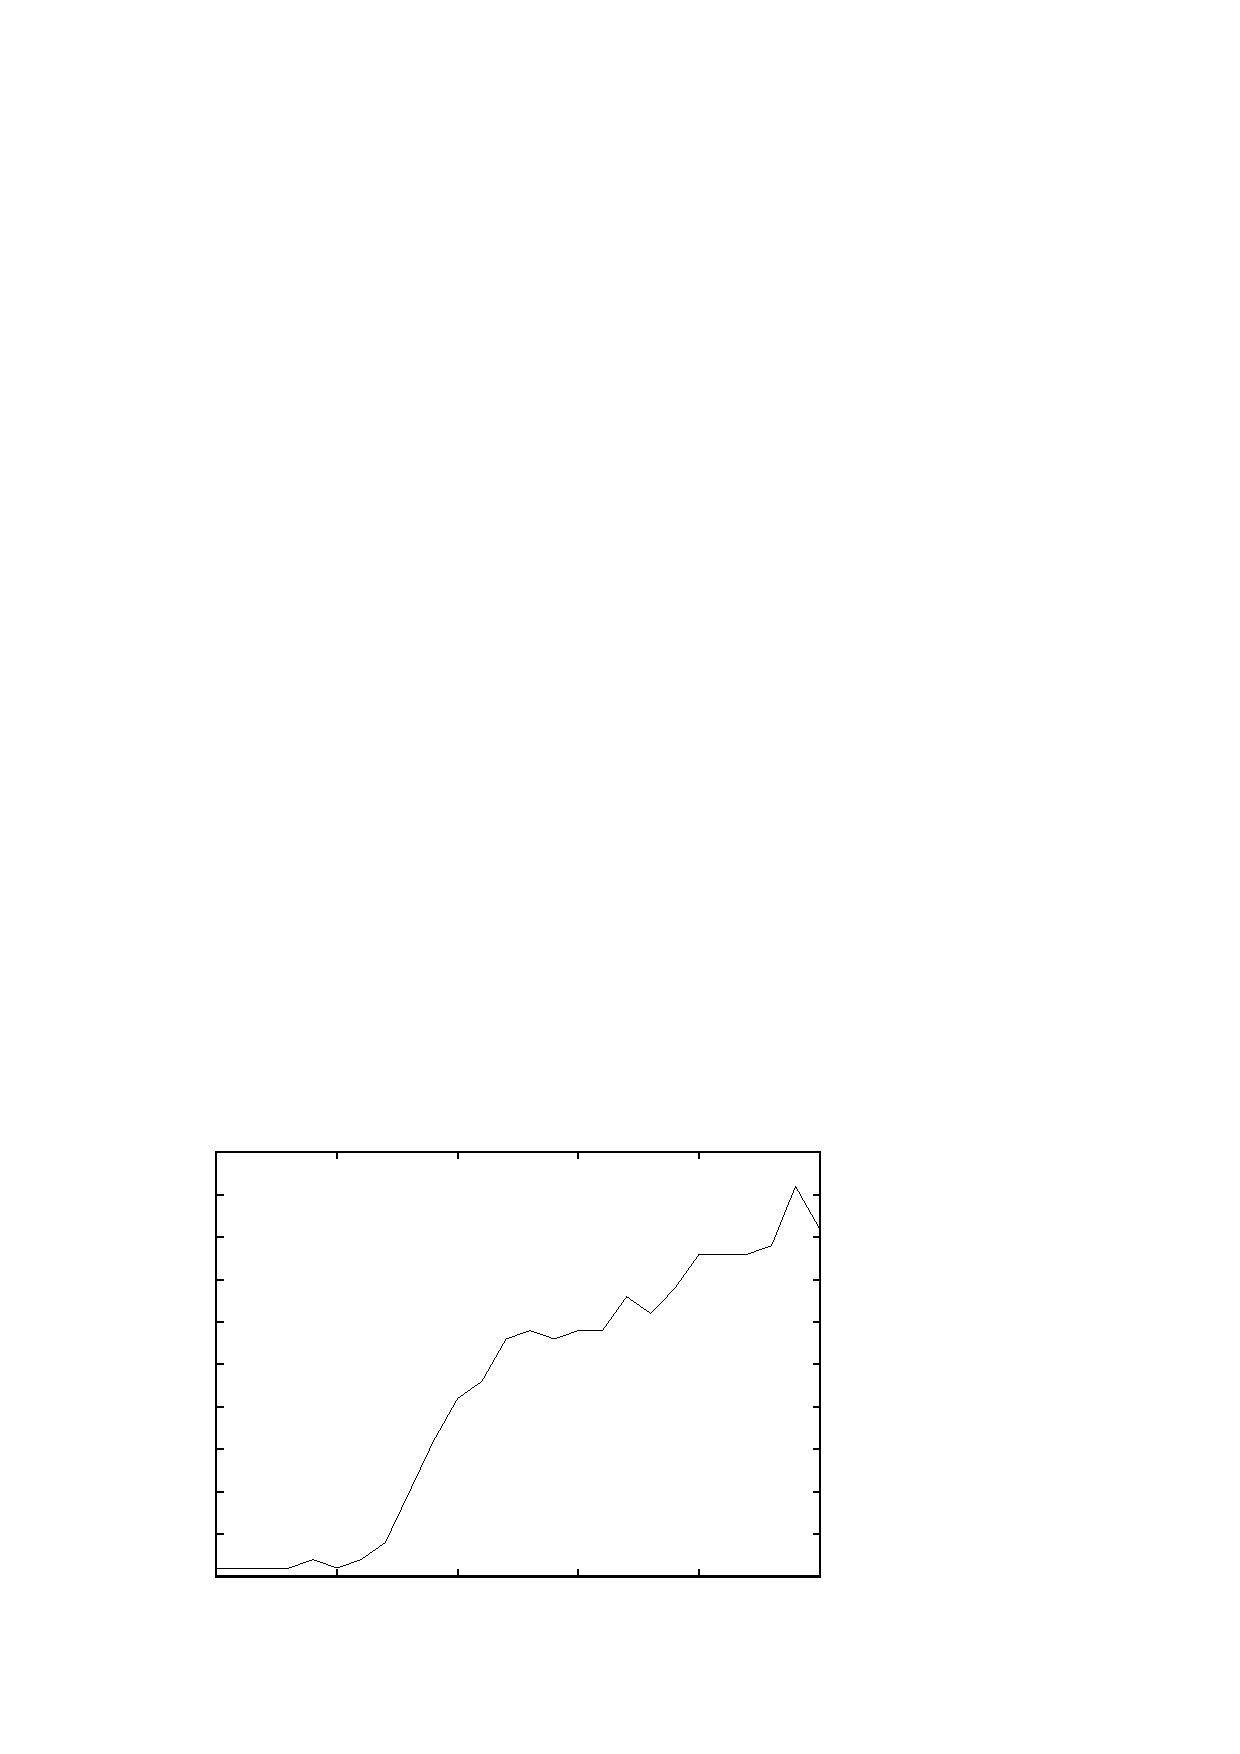
\includegraphics{Cu15brz}}%
    \gplfronttext
  \end{picture}%
\endgroup

\end{center}
\caption{Oblast brzdného spektra rengenky s Cu anodou při napětí 15 kV a expozicí 8 s.}
\label{prvni}
\end{figure}

\begin{figure}
\begin{center}
% GNUPLOT: LaTeX picture with Postscript
\begingroup
  \makeatletter
  \providecommand\color[2][]{%
    \GenericError{(gnuplot) \space\space\space\@spaces}{%
      Package color not loaded in conjunction with
      terminal option `colourtext'%
    }{See the gnuplot documentation for explanation.%
    }{Either use 'blacktext' in gnuplot or load the package
      color.sty in LaTeX.}%
    \renewcommand\color[2][]{}%
  }%
  \providecommand\includegraphics[2][]{%
    \GenericError{(gnuplot) \space\space\space\@spaces}{%
      Package graphicx or graphics not loaded%
    }{See the gnuplot documentation for explanation.%
    }{The gnuplot epslatex terminal needs graphicx.sty or graphics.sty.}%
    \renewcommand\includegraphics[2][]{}%
  }%
  \providecommand\rotatebox[2]{#2}%
  \@ifundefined{ifGPcolor}{%
    \newif\ifGPcolor
    \GPcolorfalse
  }{}%
  \@ifundefined{ifGPblacktext}{%
    \newif\ifGPblacktext
    \GPblacktexttrue
  }{}%
  % define a \g@addto@macro without @ in the name:
  \let\gplgaddtomacro\g@addto@macro
  % define empty templates for all commands taking text:
  \gdef\gplbacktext{}%
  \gdef\gplfronttext{}%
  \makeatother
  \ifGPblacktext
    % no textcolor at all
    \def\colorrgb#1{}%
    \def\colorgray#1{}%
  \else
    % gray or color?
    \ifGPcolor
      \def\colorrgb#1{\color[rgb]{#1}}%
      \def\colorgray#1{\color[gray]{#1}}%
      \expandafter\def\csname LTw\endcsname{\color{white}}%
      \expandafter\def\csname LTb\endcsname{\color{black}}%
      \expandafter\def\csname LTa\endcsname{\color{black}}%
      \expandafter\def\csname LT0\endcsname{\color[rgb]{1,0,0}}%
      \expandafter\def\csname LT1\endcsname{\color[rgb]{0,1,0}}%
      \expandafter\def\csname LT2\endcsname{\color[rgb]{0,0,1}}%
      \expandafter\def\csname LT3\endcsname{\color[rgb]{1,0,1}}%
      \expandafter\def\csname LT4\endcsname{\color[rgb]{0,1,1}}%
      \expandafter\def\csname LT5\endcsname{\color[rgb]{1,1,0}}%
      \expandafter\def\csname LT6\endcsname{\color[rgb]{0,0,0}}%
      \expandafter\def\csname LT7\endcsname{\color[rgb]{1,0.3,0}}%
      \expandafter\def\csname LT8\endcsname{\color[rgb]{0.5,0.5,0.5}}%
    \else
      % gray
      \def\colorrgb#1{\color{black}}%
      \def\colorgray#1{\color[gray]{#1}}%
      \expandafter\def\csname LTw\endcsname{\color{white}}%
      \expandafter\def\csname LTb\endcsname{\color{black}}%
      \expandafter\def\csname LTa\endcsname{\color{black}}%
      \expandafter\def\csname LT0\endcsname{\color{black}}%
      \expandafter\def\csname LT1\endcsname{\color{black}}%
      \expandafter\def\csname LT2\endcsname{\color{black}}%
      \expandafter\def\csname LT3\endcsname{\color{black}}%
      \expandafter\def\csname LT4\endcsname{\color{black}}%
      \expandafter\def\csname LT5\endcsname{\color{black}}%
      \expandafter\def\csname LT6\endcsname{\color{black}}%
      \expandafter\def\csname LT7\endcsname{\color{black}}%
      \expandafter\def\csname LT8\endcsname{\color{black}}%
    \fi
  \fi
  \setlength{\unitlength}{0.0500bp}%
  \begin{picture}(7200.00,5040.00)%
    \gplgaddtomacro\gplbacktext{%
      \csname LTb\endcsname%
      \put(1078,704){\makebox(0,0)[r]{\strut{} 0}}%
      \put(1078,1286){\makebox(0,0)[r]{\strut{} 20}}%
      \put(1078,1867){\makebox(0,0)[r]{\strut{} 40}}%
      \put(1078,2449){\makebox(0,0)[r]{\strut{} 60}}%
      \put(1078,3030){\makebox(0,0)[r]{\strut{} 80}}%
      \put(1078,3612){\makebox(0,0)[r]{\strut{} 100}}%
      \put(1078,4193){\makebox(0,0)[r]{\strut{} 120}}%
      \put(1078,4775){\makebox(0,0)[r]{\strut{} 140}}%
      \put(1210,484){\makebox(0,0){\strut{} 3}}%
      \put(2018,484){\makebox(0,0){\strut{} 4}}%
      \put(2827,484){\makebox(0,0){\strut{} 5}}%
      \put(3635,484){\makebox(0,0){\strut{} 6}}%
      \put(4444,484){\makebox(0,0){\strut{} 7}}%
      \put(5252,484){\makebox(0,0){\strut{} 8}}%
      \put(6061,484){\makebox(0,0){\strut{} 9}}%
      \put(6869,484){\makebox(0,0){\strut{} 10}}%
      \put(308,2739){\rotatebox{-270}{\makebox(0,0){\strut{}Imp/s}}}%
      \put(4039,154){\makebox(0,0){\strut{}$\theta$/\st}}%
    }%
    \gplgaddtomacro\gplfronttext{%
    }%
    \gplbacktext
    \put(0,0){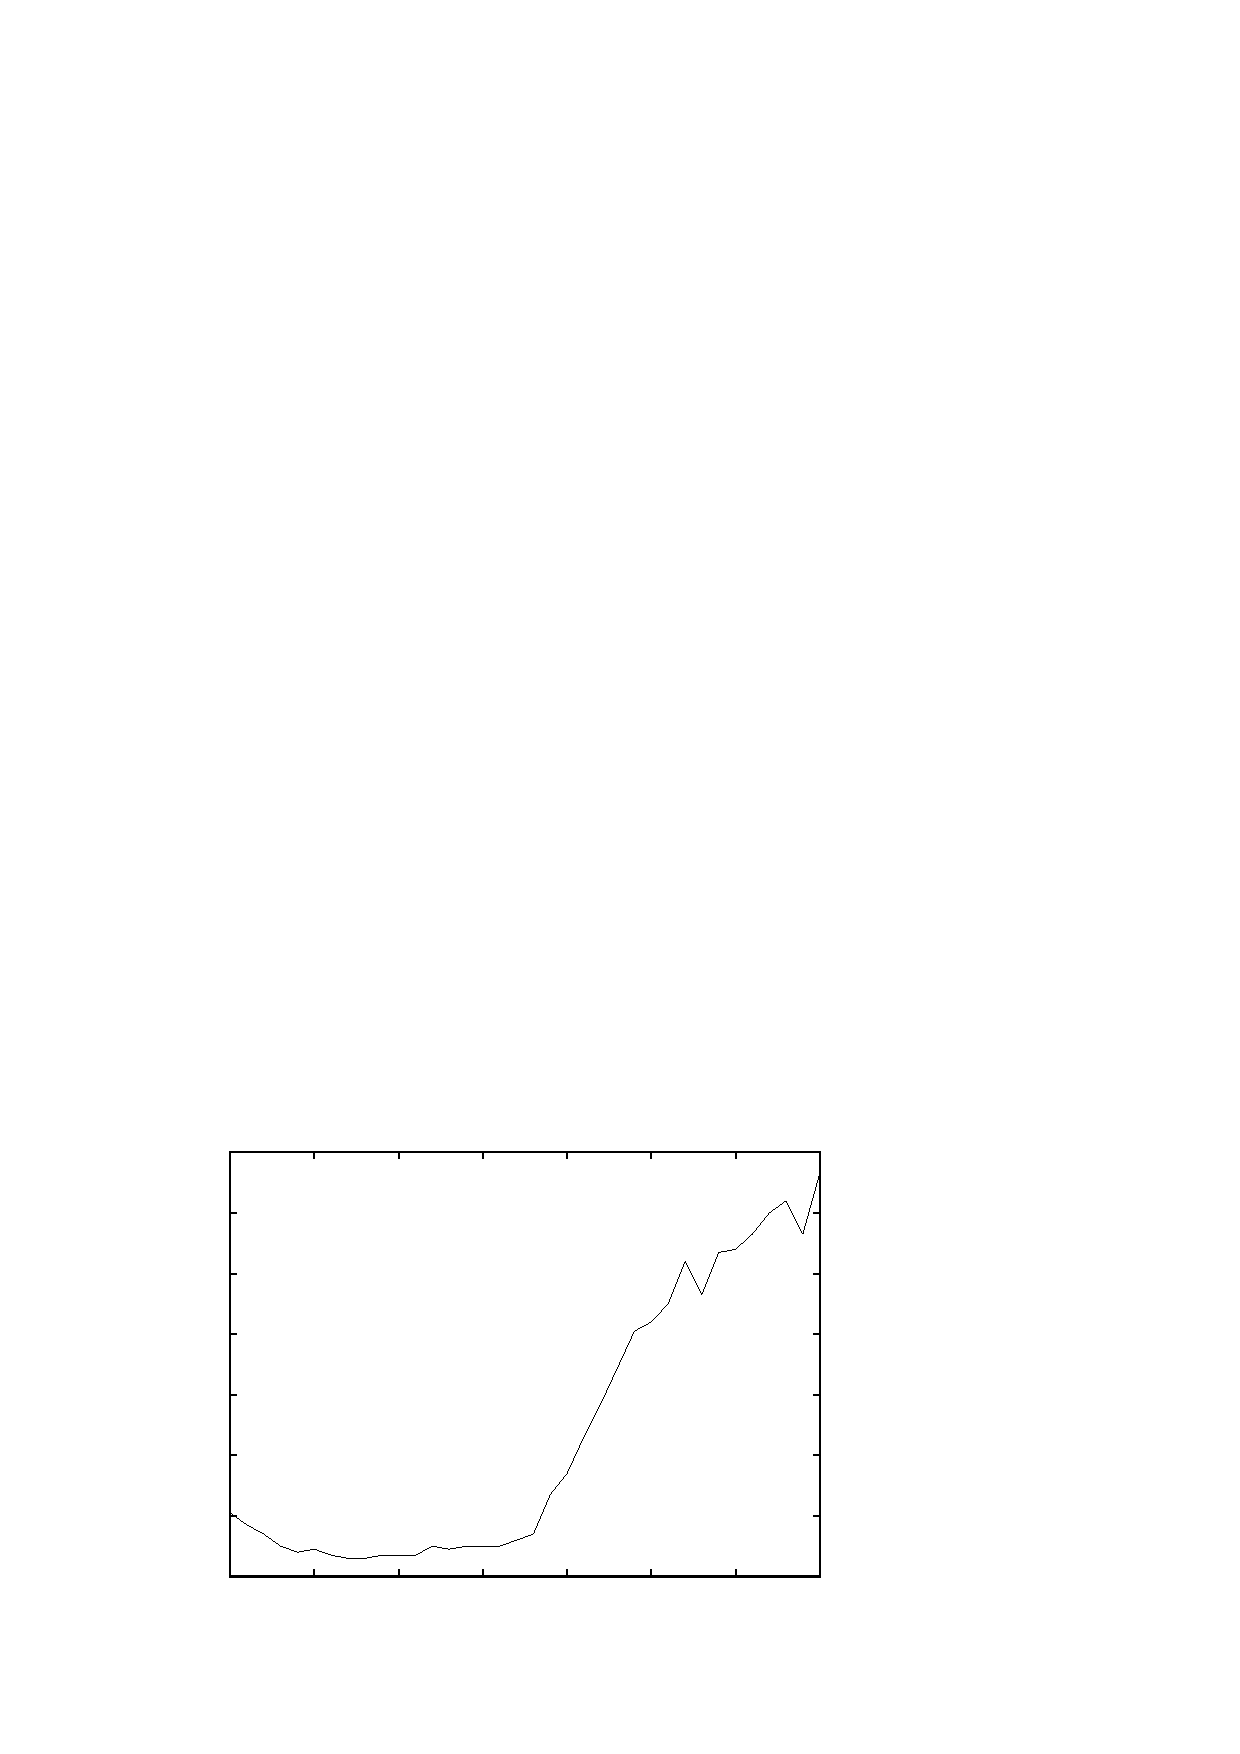
\includegraphics{Cu25brz}}%
    \gplfronttext
  \end{picture}%
\endgroup

\end{center}
\caption{Oblast brzdného spektra rengenky s Cu anodou při napětí 25 kV a expozicí 5 s.}
\end{figure}

\begin{figure}
\begin{center}
% GNUPLOT: LaTeX picture with Postscript
\begingroup
  \makeatletter
  \providecommand\color[2][]{%
    \GenericError{(gnuplot) \space\space\space\@spaces}{%
      Package color not loaded in conjunction with
      terminal option `colourtext'%
    }{See the gnuplot documentation for explanation.%
    }{Either use 'blacktext' in gnuplot or load the package
      color.sty in LaTeX.}%
    \renewcommand\color[2][]{}%
  }%
  \providecommand\includegraphics[2][]{%
    \GenericError{(gnuplot) \space\space\space\@spaces}{%
      Package graphicx or graphics not loaded%
    }{See the gnuplot documentation for explanation.%
    }{The gnuplot epslatex terminal needs graphicx.sty or graphics.sty.}%
    \renewcommand\includegraphics[2][]{}%
  }%
  \providecommand\rotatebox[2]{#2}%
  \@ifundefined{ifGPcolor}{%
    \newif\ifGPcolor
    \GPcolorfalse
  }{}%
  \@ifundefined{ifGPblacktext}{%
    \newif\ifGPblacktext
    \GPblacktexttrue
  }{}%
  % define a \g@addto@macro without @ in the name:
  \let\gplgaddtomacro\g@addto@macro
  % define empty templates for all commands taking text:
  \gdef\gplbacktext{}%
  \gdef\gplfronttext{}%
  \makeatother
  \ifGPblacktext
    % no textcolor at all
    \def\colorrgb#1{}%
    \def\colorgray#1{}%
  \else
    % gray or color?
    \ifGPcolor
      \def\colorrgb#1{\color[rgb]{#1}}%
      \def\colorgray#1{\color[gray]{#1}}%
      \expandafter\def\csname LTw\endcsname{\color{white}}%
      \expandafter\def\csname LTb\endcsname{\color{black}}%
      \expandafter\def\csname LTa\endcsname{\color{black}}%
      \expandafter\def\csname LT0\endcsname{\color[rgb]{1,0,0}}%
      \expandafter\def\csname LT1\endcsname{\color[rgb]{0,1,0}}%
      \expandafter\def\csname LT2\endcsname{\color[rgb]{0,0,1}}%
      \expandafter\def\csname LT3\endcsname{\color[rgb]{1,0,1}}%
      \expandafter\def\csname LT4\endcsname{\color[rgb]{0,1,1}}%
      \expandafter\def\csname LT5\endcsname{\color[rgb]{1,1,0}}%
      \expandafter\def\csname LT6\endcsname{\color[rgb]{0,0,0}}%
      \expandafter\def\csname LT7\endcsname{\color[rgb]{1,0.3,0}}%
      \expandafter\def\csname LT8\endcsname{\color[rgb]{0.5,0.5,0.5}}%
    \else
      % gray
      \def\colorrgb#1{\color{black}}%
      \def\colorgray#1{\color[gray]{#1}}%
      \expandafter\def\csname LTw\endcsname{\color{white}}%
      \expandafter\def\csname LTb\endcsname{\color{black}}%
      \expandafter\def\csname LTa\endcsname{\color{black}}%
      \expandafter\def\csname LT0\endcsname{\color{black}}%
      \expandafter\def\csname LT1\endcsname{\color{black}}%
      \expandafter\def\csname LT2\endcsname{\color{black}}%
      \expandafter\def\csname LT3\endcsname{\color{black}}%
      \expandafter\def\csname LT4\endcsname{\color{black}}%
      \expandafter\def\csname LT5\endcsname{\color{black}}%
      \expandafter\def\csname LT6\endcsname{\color{black}}%
      \expandafter\def\csname LT7\endcsname{\color{black}}%
      \expandafter\def\csname LT8\endcsname{\color{black}}%
    \fi
  \fi
  \setlength{\unitlength}{0.0500bp}%
  \begin{picture}(7200.00,5040.00)%
    \gplgaddtomacro\gplbacktext{%
      \csname LTb\endcsname%
      \put(1078,704){\makebox(0,0)[r]{\strut{} 0}}%
      \put(1078,1074){\makebox(0,0)[r]{\strut{} 20}}%
      \put(1078,1444){\makebox(0,0)[r]{\strut{} 40}}%
      \put(1078,1814){\makebox(0,0)[r]{\strut{} 60}}%
      \put(1078,2184){\makebox(0,0)[r]{\strut{} 80}}%
      \put(1078,2554){\makebox(0,0)[r]{\strut{} 100}}%
      \put(1078,2925){\makebox(0,0)[r]{\strut{} 120}}%
      \put(1078,3295){\makebox(0,0)[r]{\strut{} 140}}%
      \put(1078,3665){\makebox(0,0)[r]{\strut{} 160}}%
      \put(1078,4035){\makebox(0,0)[r]{\strut{} 180}}%
      \put(1078,4405){\makebox(0,0)[r]{\strut{} 200}}%
      \put(1078,4775){\makebox(0,0)[r]{\strut{} 220}}%
      \put(1210,484){\makebox(0,0){\strut{} 3}}%
      \put(2018,484){\makebox(0,0){\strut{} 4}}%
      \put(2827,484){\makebox(0,0){\strut{} 5}}%
      \put(3635,484){\makebox(0,0){\strut{} 6}}%
      \put(4444,484){\makebox(0,0){\strut{} 7}}%
      \put(5252,484){\makebox(0,0){\strut{} 8}}%
      \put(6061,484){\makebox(0,0){\strut{} 9}}%
      \put(6869,484){\makebox(0,0){\strut{} 10}}%
      \put(308,2739){\rotatebox{-270}{\makebox(0,0){\strut{}Imp/s}}}%
      \put(4039,154){\makebox(0,0){\strut{}$\theta$/\st}}%
    }%
    \gplgaddtomacro\gplfronttext{%
    }%
    \gplbacktext
    \put(0,0){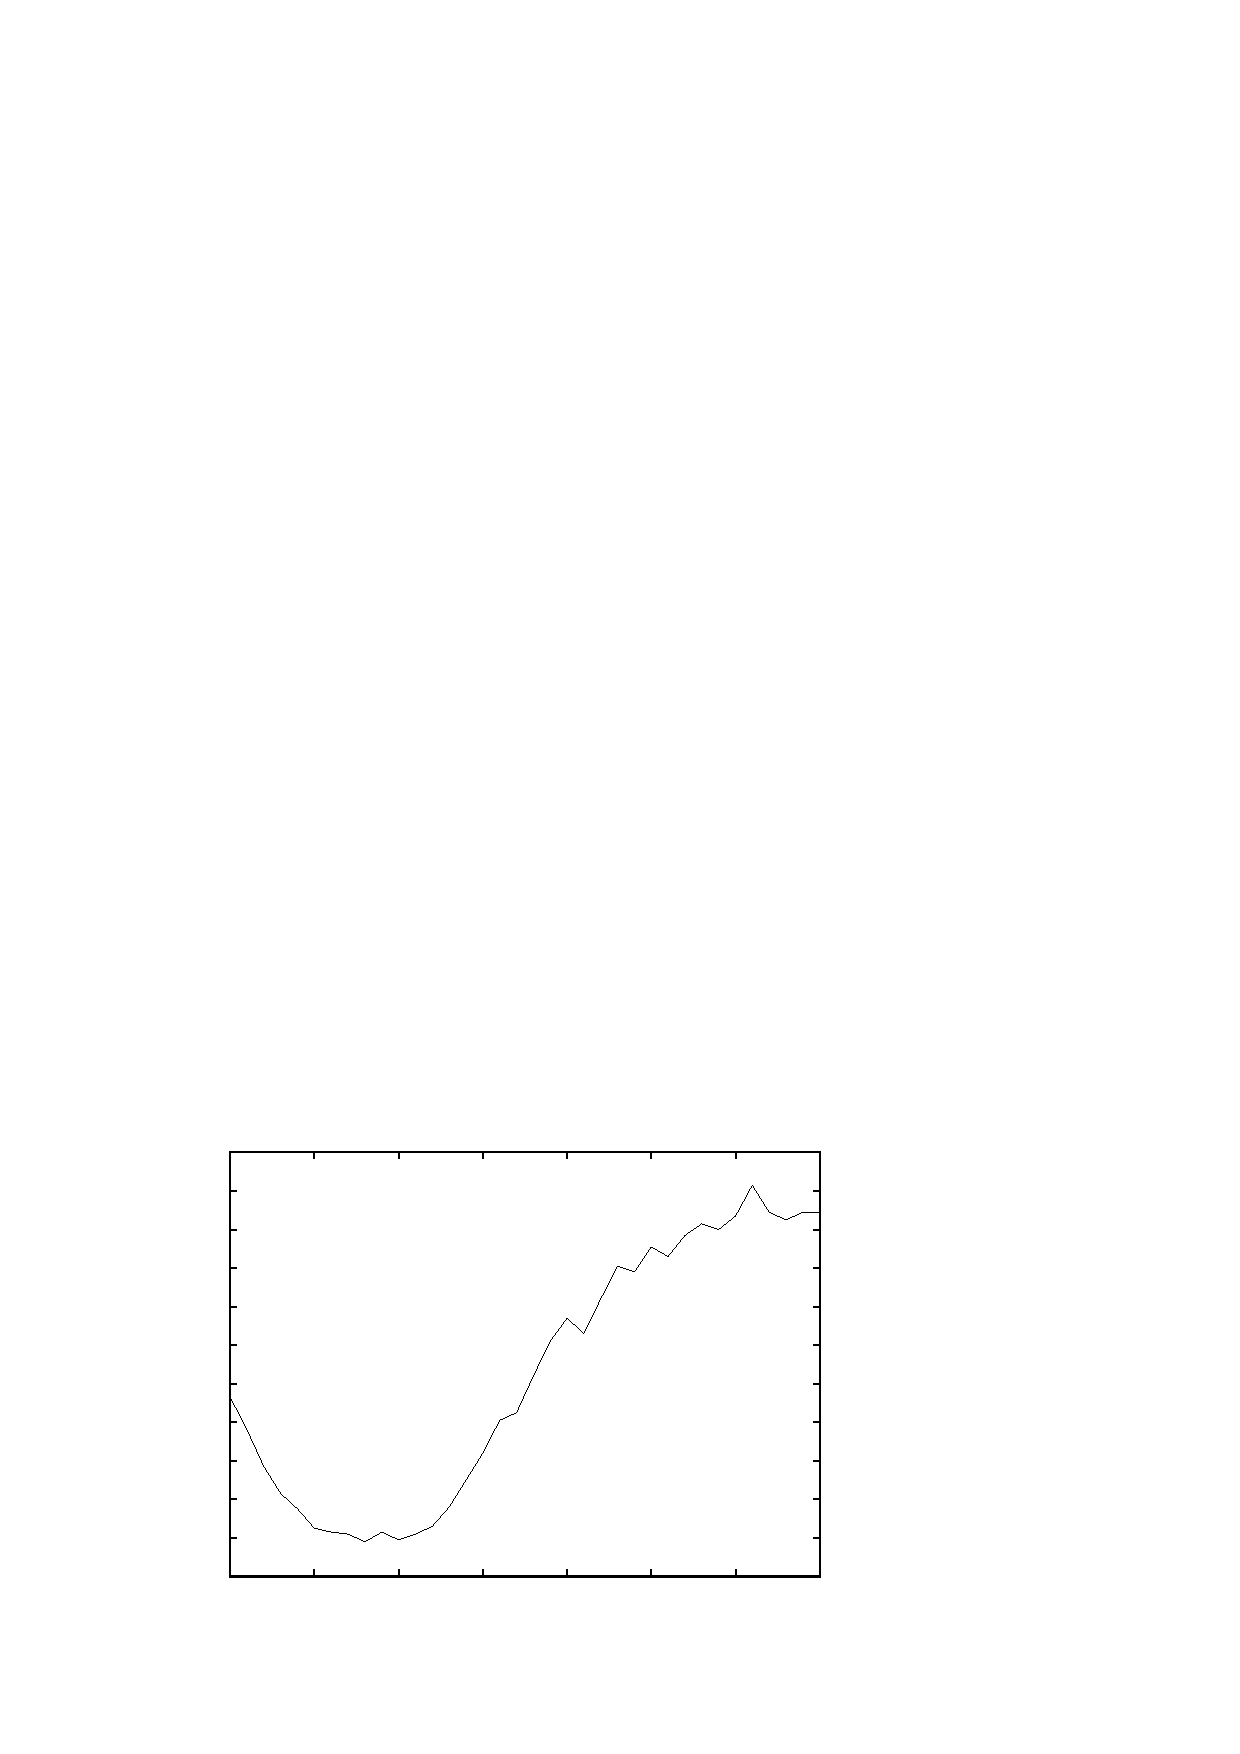
\includegraphics{Cu30brz}}%
    \gplfronttext
  \end{picture}%
\endgroup

\end{center}
\caption{Oblast brzdného spektra rengenky s Cu anodou při napětí 30 kV a expozicí 5 s.}
\end{figure}

\begin{figure}
\begin{center}
% GNUPLOT: LaTeX picture with Postscript
\begingroup
  \makeatletter
  \providecommand\color[2][]{%
    \GenericError{(gnuplot) \space\space\space\@spaces}{%
      Package color not loaded in conjunction with
      terminal option `colourtext'%
    }{See the gnuplot documentation for explanation.%
    }{Either use 'blacktext' in gnuplot or load the package
      color.sty in LaTeX.}%
    \renewcommand\color[2][]{}%
  }%
  \providecommand\includegraphics[2][]{%
    \GenericError{(gnuplot) \space\space\space\@spaces}{%
      Package graphicx or graphics not loaded%
    }{See the gnuplot documentation for explanation.%
    }{The gnuplot epslatex terminal needs graphicx.sty or graphics.sty.}%
    \renewcommand\includegraphics[2][]{}%
  }%
  \providecommand\rotatebox[2]{#2}%
  \@ifundefined{ifGPcolor}{%
    \newif\ifGPcolor
    \GPcolorfalse
  }{}%
  \@ifundefined{ifGPblacktext}{%
    \newif\ifGPblacktext
    \GPblacktexttrue
  }{}%
  % define a \g@addto@macro without @ in the name:
  \let\gplgaddtomacro\g@addto@macro
  % define empty templates for all commands taking text:
  \gdef\gplbacktext{}%
  \gdef\gplfronttext{}%
  \makeatother
  \ifGPblacktext
    % no textcolor at all
    \def\colorrgb#1{}%
    \def\colorgray#1{}%
  \else
    % gray or color?
    \ifGPcolor
      \def\colorrgb#1{\color[rgb]{#1}}%
      \def\colorgray#1{\color[gray]{#1}}%
      \expandafter\def\csname LTw\endcsname{\color{white}}%
      \expandafter\def\csname LTb\endcsname{\color{black}}%
      \expandafter\def\csname LTa\endcsname{\color{black}}%
      \expandafter\def\csname LT0\endcsname{\color[rgb]{1,0,0}}%
      \expandafter\def\csname LT1\endcsname{\color[rgb]{0,1,0}}%
      \expandafter\def\csname LT2\endcsname{\color[rgb]{0,0,1}}%
      \expandafter\def\csname LT3\endcsname{\color[rgb]{1,0,1}}%
      \expandafter\def\csname LT4\endcsname{\color[rgb]{0,1,1}}%
      \expandafter\def\csname LT5\endcsname{\color[rgb]{1,1,0}}%
      \expandafter\def\csname LT6\endcsname{\color[rgb]{0,0,0}}%
      \expandafter\def\csname LT7\endcsname{\color[rgb]{1,0.3,0}}%
      \expandafter\def\csname LT8\endcsname{\color[rgb]{0.5,0.5,0.5}}%
    \else
      % gray
      \def\colorrgb#1{\color{black}}%
      \def\colorgray#1{\color[gray]{#1}}%
      \expandafter\def\csname LTw\endcsname{\color{white}}%
      \expandafter\def\csname LTb\endcsname{\color{black}}%
      \expandafter\def\csname LTa\endcsname{\color{black}}%
      \expandafter\def\csname LT0\endcsname{\color{black}}%
      \expandafter\def\csname LT1\endcsname{\color{black}}%
      \expandafter\def\csname LT2\endcsname{\color{black}}%
      \expandafter\def\csname LT3\endcsname{\color{black}}%
      \expandafter\def\csname LT4\endcsname{\color{black}}%
      \expandafter\def\csname LT5\endcsname{\color{black}}%
      \expandafter\def\csname LT6\endcsname{\color{black}}%
      \expandafter\def\csname LT7\endcsname{\color{black}}%
      \expandafter\def\csname LT8\endcsname{\color{black}}%
    \fi
  \fi
  \setlength{\unitlength}{0.0500bp}%
  \begin{picture}(7200.00,5040.00)%
    \gplgaddtomacro\gplbacktext{%
      \csname LTb\endcsname%
      \put(1078,704){\makebox(0,0)[r]{\strut{} 0}}%
      \put(1078,1518){\makebox(0,0)[r]{\strut{} 50}}%
      \put(1078,2332){\makebox(0,0)[r]{\strut{} 100}}%
      \put(1078,3147){\makebox(0,0)[r]{\strut{} 150}}%
      \put(1078,3961){\makebox(0,0)[r]{\strut{} 200}}%
      \put(1078,4775){\makebox(0,0)[r]{\strut{} 250}}%
      \put(1210,484){\makebox(0,0){\strut{} 3}}%
      \put(2018,484){\makebox(0,0){\strut{} 4}}%
      \put(2827,484){\makebox(0,0){\strut{} 5}}%
      \put(3635,484){\makebox(0,0){\strut{} 6}}%
      \put(4444,484){\makebox(0,0){\strut{} 7}}%
      \put(5252,484){\makebox(0,0){\strut{} 8}}%
      \put(6061,484){\makebox(0,0){\strut{} 9}}%
      \put(6869,484){\makebox(0,0){\strut{} 10}}%
      \put(308,2739){\rotatebox{-270}{\makebox(0,0){\strut{}Imp/s}}}%
      \put(4039,154){\makebox(0,0){\strut{}$\theta$/\st}}%
    }%
    \gplgaddtomacro\gplfronttext{%
    }%
    \gplbacktext
    \put(0,0){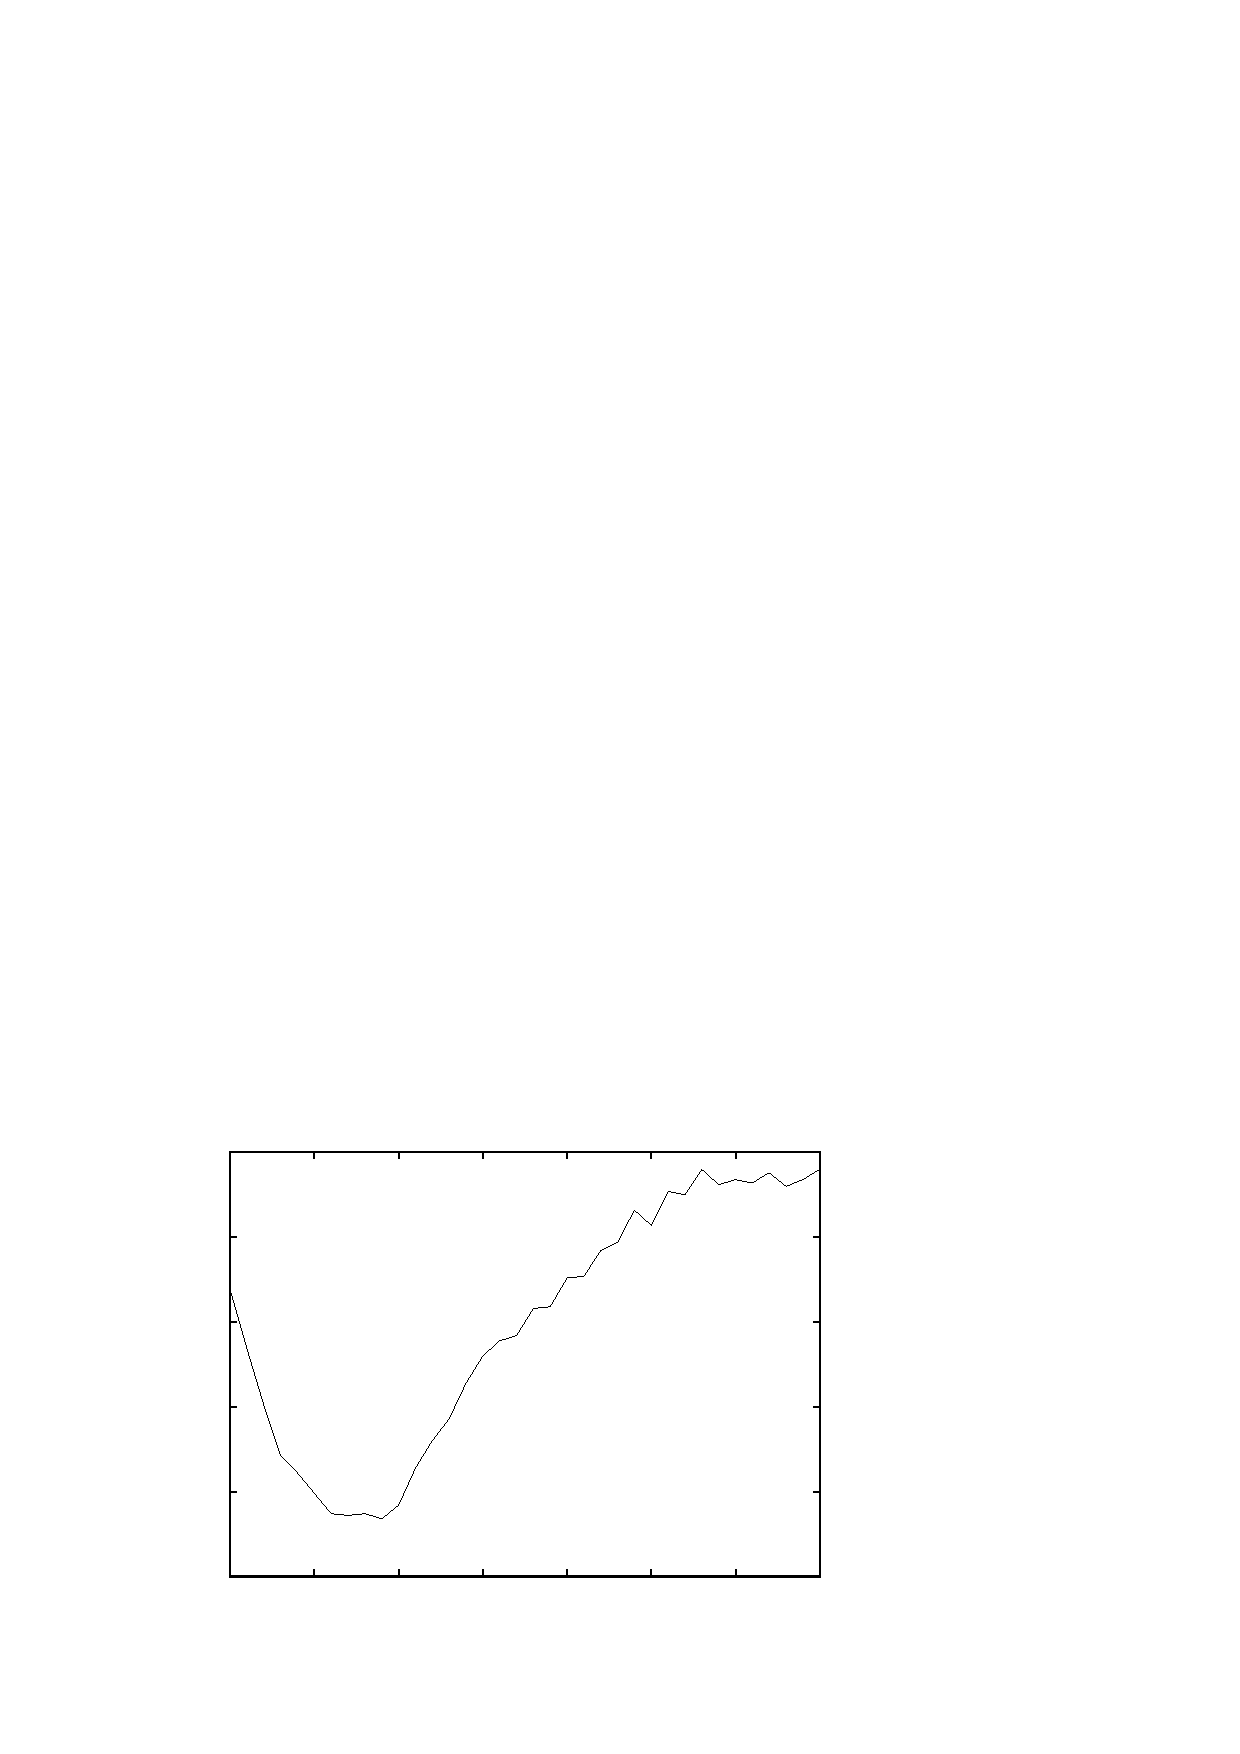
\includegraphics{Cu33brz}}%
    \gplfronttext
  \end{picture}%
\endgroup

\end{center}
\caption{Oblast brzdného spektra rengenky s Cu anodou při napětí 15 kV a expozicí 5 s.}
\end{figure}

\begin{figure}
\begin{center}
% GNUPLOT: LaTeX picture with Postscript
\begingroup
  \makeatletter
  \providecommand\color[2][]{%
    \GenericError{(gnuplot) \space\space\space\@spaces}{%
      Package color not loaded in conjunction with
      terminal option `colourtext'%
    }{See the gnuplot documentation for explanation.%
    }{Either use 'blacktext' in gnuplot or load the package
      color.sty in LaTeX.}%
    \renewcommand\color[2][]{}%
  }%
  \providecommand\includegraphics[2][]{%
    \GenericError{(gnuplot) \space\space\space\@spaces}{%
      Package graphicx or graphics not loaded%
    }{See the gnuplot documentation for explanation.%
    }{The gnuplot epslatex terminal needs graphicx.sty or graphics.sty.}%
    \renewcommand\includegraphics[2][]{}%
  }%
  \providecommand\rotatebox[2]{#2}%
  \@ifundefined{ifGPcolor}{%
    \newif\ifGPcolor
    \GPcolorfalse
  }{}%
  \@ifundefined{ifGPblacktext}{%
    \newif\ifGPblacktext
    \GPblacktexttrue
  }{}%
  % define a \g@addto@macro without @ in the name:
  \let\gplgaddtomacro\g@addto@macro
  % define empty templates for all commands taking text:
  \gdef\gplbacktext{}%
  \gdef\gplfronttext{}%
  \makeatother
  \ifGPblacktext
    % no textcolor at all
    \def\colorrgb#1{}%
    \def\colorgray#1{}%
  \else
    % gray or color?
    \ifGPcolor
      \def\colorrgb#1{\color[rgb]{#1}}%
      \def\colorgray#1{\color[gray]{#1}}%
      \expandafter\def\csname LTw\endcsname{\color{white}}%
      \expandafter\def\csname LTb\endcsname{\color{black}}%
      \expandafter\def\csname LTa\endcsname{\color{black}}%
      \expandafter\def\csname LT0\endcsname{\color[rgb]{1,0,0}}%
      \expandafter\def\csname LT1\endcsname{\color[rgb]{0,1,0}}%
      \expandafter\def\csname LT2\endcsname{\color[rgb]{0,0,1}}%
      \expandafter\def\csname LT3\endcsname{\color[rgb]{1,0,1}}%
      \expandafter\def\csname LT4\endcsname{\color[rgb]{0,1,1}}%
      \expandafter\def\csname LT5\endcsname{\color[rgb]{1,1,0}}%
      \expandafter\def\csname LT6\endcsname{\color[rgb]{0,0,0}}%
      \expandafter\def\csname LT7\endcsname{\color[rgb]{1,0.3,0}}%
      \expandafter\def\csname LT8\endcsname{\color[rgb]{0.5,0.5,0.5}}%
    \else
      % gray
      \def\colorrgb#1{\color{black}}%
      \def\colorgray#1{\color[gray]{#1}}%
      \expandafter\def\csname LTw\endcsname{\color{white}}%
      \expandafter\def\csname LTb\endcsname{\color{black}}%
      \expandafter\def\csname LTa\endcsname{\color{black}}%
      \expandafter\def\csname LT0\endcsname{\color{black}}%
      \expandafter\def\csname LT1\endcsname{\color{black}}%
      \expandafter\def\csname LT2\endcsname{\color{black}}%
      \expandafter\def\csname LT3\endcsname{\color{black}}%
      \expandafter\def\csname LT4\endcsname{\color{black}}%
      \expandafter\def\csname LT5\endcsname{\color{black}}%
      \expandafter\def\csname LT6\endcsname{\color{black}}%
      \expandafter\def\csname LT7\endcsname{\color{black}}%
      \expandafter\def\csname LT8\endcsname{\color{black}}%
    \fi
  \fi
  \setlength{\unitlength}{0.0500bp}%
  \begin{picture}(7200.00,5040.00)%
    \gplgaddtomacro\gplbacktext{%
      \csname LTb\endcsname%
      \put(1210,704){\makebox(0,0)[r]{\strut{} 0}}%
      \put(1210,1286){\makebox(0,0)[r]{\strut{} 200}}%
      \put(1210,1867){\makebox(0,0)[r]{\strut{} 400}}%
      \put(1210,2449){\makebox(0,0)[r]{\strut{} 600}}%
      \put(1210,3030){\makebox(0,0)[r]{\strut{} 800}}%
      \put(1210,3612){\makebox(0,0)[r]{\strut{} 1000}}%
      \put(1210,4193){\makebox(0,0)[r]{\strut{} 1200}}%
      \put(1210,4775){\makebox(0,0)[r]{\strut{} 1400}}%
      \put(1342,484){\makebox(0,0){\strut{} 14}}%
      \put(2033,484){\makebox(0,0){\strut{} 16}}%
      \put(2724,484){\makebox(0,0){\strut{} 18}}%
      \put(3415,484){\makebox(0,0){\strut{} 20}}%
      \put(4106,484){\makebox(0,0){\strut{} 22}}%
      \put(4796,484){\makebox(0,0){\strut{} 24}}%
      \put(5487,484){\makebox(0,0){\strut{} 26}}%
      \put(6178,484){\makebox(0,0){\strut{} 28}}%
      \put(6869,484){\makebox(0,0){\strut{} 30}}%
      \put(308,2739){\rotatebox{-270}{\makebox(0,0){\strut{}Imp/s}}}%
      \put(4105,154){\makebox(0,0){\strut{}$\theta$/\st}}%
    }%
    \gplgaddtomacro\gplfronttext{%
    }%
    \gplbacktext
    \put(0,0){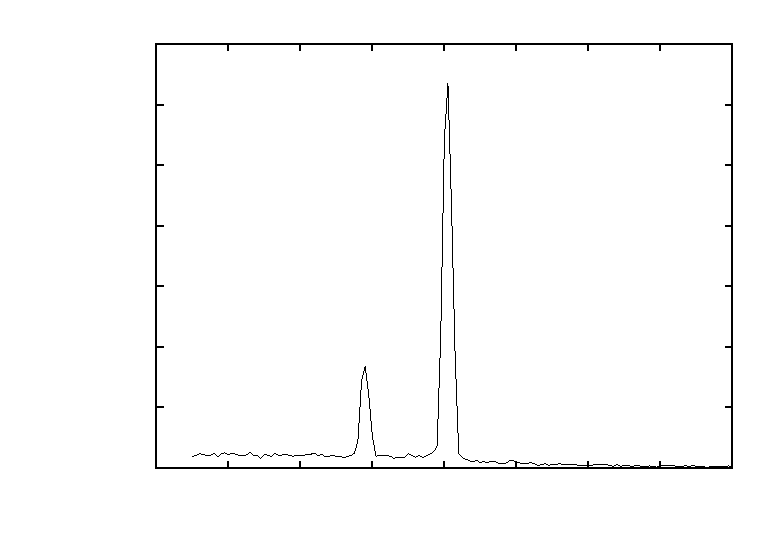
\includegraphics{Cu15sp}}%
    \gplfronttext
  \end{picture}%
\endgroup

\end{center}
\caption{Oblast specifického záření pro rengenku s Cu anodou při napětí 15 kV a expozicí 2 s.}
\end{figure}

\begin{figure}
\begin{center}
% GNUPLOT: LaTeX picture with Postscript
\begingroup
  \makeatletter
  \providecommand\color[2][]{%
    \GenericError{(gnuplot) \space\space\space\@spaces}{%
      Package color not loaded in conjunction with
      terminal option `colourtext'%
    }{See the gnuplot documentation for explanation.%
    }{Either use 'blacktext' in gnuplot or load the package
      color.sty in LaTeX.}%
    \renewcommand\color[2][]{}%
  }%
  \providecommand\includegraphics[2][]{%
    \GenericError{(gnuplot) \space\space\space\@spaces}{%
      Package graphicx or graphics not loaded%
    }{See the gnuplot documentation for explanation.%
    }{The gnuplot epslatex terminal needs graphicx.sty or graphics.sty.}%
    \renewcommand\includegraphics[2][]{}%
  }%
  \providecommand\rotatebox[2]{#2}%
  \@ifundefined{ifGPcolor}{%
    \newif\ifGPcolor
    \GPcolorfalse
  }{}%
  \@ifundefined{ifGPblacktext}{%
    \newif\ifGPblacktext
    \GPblacktexttrue
  }{}%
  % define a \g@addto@macro without @ in the name:
  \let\gplgaddtomacro\g@addto@macro
  % define empty templates for all commands taking text:
  \gdef\gplbacktext{}%
  \gdef\gplfronttext{}%
  \makeatother
  \ifGPblacktext
    % no textcolor at all
    \def\colorrgb#1{}%
    \def\colorgray#1{}%
  \else
    % gray or color?
    \ifGPcolor
      \def\colorrgb#1{\color[rgb]{#1}}%
      \def\colorgray#1{\color[gray]{#1}}%
      \expandafter\def\csname LTw\endcsname{\color{white}}%
      \expandafter\def\csname LTb\endcsname{\color{black}}%
      \expandafter\def\csname LTa\endcsname{\color{black}}%
      \expandafter\def\csname LT0\endcsname{\color[rgb]{1,0,0}}%
      \expandafter\def\csname LT1\endcsname{\color[rgb]{0,1,0}}%
      \expandafter\def\csname LT2\endcsname{\color[rgb]{0,0,1}}%
      \expandafter\def\csname LT3\endcsname{\color[rgb]{1,0,1}}%
      \expandafter\def\csname LT4\endcsname{\color[rgb]{0,1,1}}%
      \expandafter\def\csname LT5\endcsname{\color[rgb]{1,1,0}}%
      \expandafter\def\csname LT6\endcsname{\color[rgb]{0,0,0}}%
      \expandafter\def\csname LT7\endcsname{\color[rgb]{1,0.3,0}}%
      \expandafter\def\csname LT8\endcsname{\color[rgb]{0.5,0.5,0.5}}%
    \else
      % gray
      \def\colorrgb#1{\color{black}}%
      \def\colorgray#1{\color[gray]{#1}}%
      \expandafter\def\csname LTw\endcsname{\color{white}}%
      \expandafter\def\csname LTb\endcsname{\color{black}}%
      \expandafter\def\csname LTa\endcsname{\color{black}}%
      \expandafter\def\csname LT0\endcsname{\color{black}}%
      \expandafter\def\csname LT1\endcsname{\color{black}}%
      \expandafter\def\csname LT2\endcsname{\color{black}}%
      \expandafter\def\csname LT3\endcsname{\color{black}}%
      \expandafter\def\csname LT4\endcsname{\color{black}}%
      \expandafter\def\csname LT5\endcsname{\color{black}}%
      \expandafter\def\csname LT6\endcsname{\color{black}}%
      \expandafter\def\csname LT7\endcsname{\color{black}}%
      \expandafter\def\csname LT8\endcsname{\color{black}}%
    \fi
  \fi
  \setlength{\unitlength}{0.0500bp}%
  \begin{picture}(7200.00,5040.00)%
    \gplgaddtomacro\gplbacktext{%
      \csname LTb\endcsname%
      \put(1210,704){\makebox(0,0)[r]{\strut{} 0}}%
      \put(1210,1286){\makebox(0,0)[r]{\strut{} 1000}}%
      \put(1210,1867){\makebox(0,0)[r]{\strut{} 2000}}%
      \put(1210,2449){\makebox(0,0)[r]{\strut{} 3000}}%
      \put(1210,3030){\makebox(0,0)[r]{\strut{} 4000}}%
      \put(1210,3612){\makebox(0,0)[r]{\strut{} 5000}}%
      \put(1210,4193){\makebox(0,0)[r]{\strut{} 6000}}%
      \put(1210,4775){\makebox(0,0)[r]{\strut{} 7000}}%
      \put(1342,484){\makebox(0,0){\strut{} 14}}%
      \put(2033,484){\makebox(0,0){\strut{} 16}}%
      \put(2724,484){\makebox(0,0){\strut{} 18}}%
      \put(3415,484){\makebox(0,0){\strut{} 20}}%
      \put(4106,484){\makebox(0,0){\strut{} 22}}%
      \put(4796,484){\makebox(0,0){\strut{} 24}}%
      \put(5487,484){\makebox(0,0){\strut{} 26}}%
      \put(6178,484){\makebox(0,0){\strut{} 28}}%
      \put(6869,484){\makebox(0,0){\strut{} 30}}%
      \put(308,2739){\rotatebox{-270}{\makebox(0,0){\strut{}Imp/s}}}%
      \put(4105,154){\makebox(0,0){\strut{}$\theta$/\st}}%
    }%
    \gplgaddtomacro\gplfronttext{%
    }%
    \gplbacktext
    \put(0,0){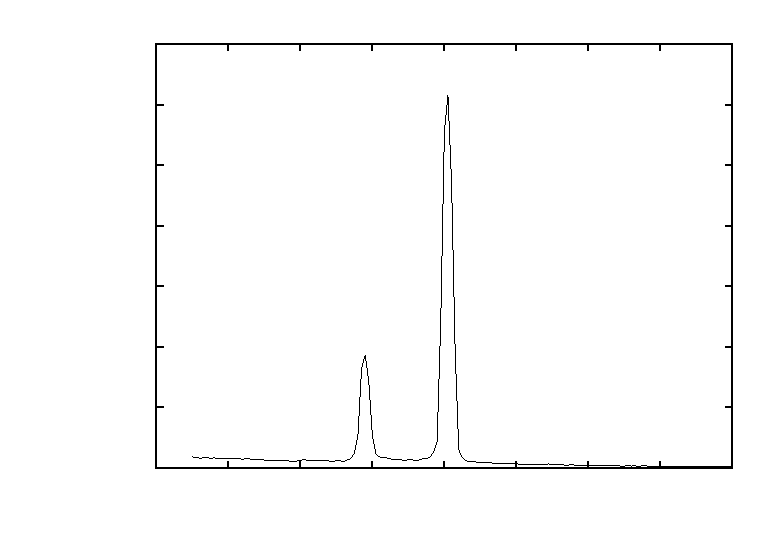
\includegraphics{Cu33sp}}%
    \gplfronttext
  \end{picture}%
\endgroup

\end{center}
\caption{Oblast specifického záření pro rengenku s Cu anodou při napětí 33 kV a expozicí 2 s.}
\end{figure}

\begin{figure}
\begin{center}
% GNUPLOT: LaTeX picture with Postscript
\begingroup
  \makeatletter
  \providecommand\color[2][]{%
    \GenericError{(gnuplot) \space\space\space\@spaces}{%
      Package color not loaded in conjunction with
      terminal option `colourtext'%
    }{See the gnuplot documentation for explanation.%
    }{Either use 'blacktext' in gnuplot or load the package
      color.sty in LaTeX.}%
    \renewcommand\color[2][]{}%
  }%
  \providecommand\includegraphics[2][]{%
    \GenericError{(gnuplot) \space\space\space\@spaces}{%
      Package graphicx or graphics not loaded%
    }{See the gnuplot documentation for explanation.%
    }{The gnuplot epslatex terminal needs graphicx.sty or graphics.sty.}%
    \renewcommand\includegraphics[2][]{}%
  }%
  \providecommand\rotatebox[2]{#2}%
  \@ifundefined{ifGPcolor}{%
    \newif\ifGPcolor
    \GPcolorfalse
  }{}%
  \@ifundefined{ifGPblacktext}{%
    \newif\ifGPblacktext
    \GPblacktexttrue
  }{}%
  % define a \g@addto@macro without @ in the name:
  \let\gplgaddtomacro\g@addto@macro
  % define empty templates for all commands taking text:
  \gdef\gplbacktext{}%
  \gdef\gplfronttext{}%
  \makeatother
  \ifGPblacktext
    % no textcolor at all
    \def\colorrgb#1{}%
    \def\colorgray#1{}%
  \else
    % gray or color?
    \ifGPcolor
      \def\colorrgb#1{\color[rgb]{#1}}%
      \def\colorgray#1{\color[gray]{#1}}%
      \expandafter\def\csname LTw\endcsname{\color{white}}%
      \expandafter\def\csname LTb\endcsname{\color{black}}%
      \expandafter\def\csname LTa\endcsname{\color{black}}%
      \expandafter\def\csname LT0\endcsname{\color[rgb]{1,0,0}}%
      \expandafter\def\csname LT1\endcsname{\color[rgb]{0,1,0}}%
      \expandafter\def\csname LT2\endcsname{\color[rgb]{0,0,1}}%
      \expandafter\def\csname LT3\endcsname{\color[rgb]{1,0,1}}%
      \expandafter\def\csname LT4\endcsname{\color[rgb]{0,1,1}}%
      \expandafter\def\csname LT5\endcsname{\color[rgb]{1,1,0}}%
      \expandafter\def\csname LT6\endcsname{\color[rgb]{0,0,0}}%
      \expandafter\def\csname LT7\endcsname{\color[rgb]{1,0.3,0}}%
      \expandafter\def\csname LT8\endcsname{\color[rgb]{0.5,0.5,0.5}}%
    \else
      % gray
      \def\colorrgb#1{\color{black}}%
      \def\colorgray#1{\color[gray]{#1}}%
      \expandafter\def\csname LTw\endcsname{\color{white}}%
      \expandafter\def\csname LTb\endcsname{\color{black}}%
      \expandafter\def\csname LTa\endcsname{\color{black}}%
      \expandafter\def\csname LT0\endcsname{\color{black}}%
      \expandafter\def\csname LT1\endcsname{\color{black}}%
      \expandafter\def\csname LT2\endcsname{\color{black}}%
      \expandafter\def\csname LT3\endcsname{\color{black}}%
      \expandafter\def\csname LT4\endcsname{\color{black}}%
      \expandafter\def\csname LT5\endcsname{\color{black}}%
      \expandafter\def\csname LT6\endcsname{\color{black}}%
      \expandafter\def\csname LT7\endcsname{\color{black}}%
      \expandafter\def\csname LT8\endcsname{\color{black}}%
    \fi
  \fi
  \setlength{\unitlength}{0.0500bp}%
  \begin{picture}(7200.00,5040.00)%
    \gplgaddtomacro\gplbacktext{%
      \csname LTb\endcsname%
      \put(1210,704){\makebox(0,0)[r]{\strut{} 0}}%
      \put(1210,1111){\makebox(0,0)[r]{\strut{} 100}}%
      \put(1210,1518){\makebox(0,0)[r]{\strut{} 200}}%
      \put(1210,1925){\makebox(0,0)[r]{\strut{} 300}}%
      \put(1210,2332){\makebox(0,0)[r]{\strut{} 400}}%
      \put(1210,2739){\makebox(0,0)[r]{\strut{} 500}}%
      \put(1210,3147){\makebox(0,0)[r]{\strut{} 600}}%
      \put(1210,3554){\makebox(0,0)[r]{\strut{} 700}}%
      \put(1210,3961){\makebox(0,0)[r]{\strut{} 800}}%
      \put(1210,4368){\makebox(0,0)[r]{\strut{} 900}}%
      \put(1210,4775){\makebox(0,0)[r]{\strut{} 1000}}%
      \put(1342,484){\makebox(0,0){\strut{} 0}}%
      \put(2263,484){\makebox(0,0){\strut{} 5}}%
      \put(3184,484){\makebox(0,0){\strut{} 10}}%
      \put(4105,484){\makebox(0,0){\strut{} 15}}%
      \put(5027,484){\makebox(0,0){\strut{} 20}}%
      \put(5948,484){\makebox(0,0){\strut{} 25}}%
      \put(6869,484){\makebox(0,0){\strut{} 30}}%
      \put(308,2739){\rotatebox{-270}{\makebox(0,0){\strut{}Imp/s}}}%
      \put(4105,154){\makebox(0,0){\strut{}$\theta$/\st}}%
    }%
    \gplgaddtomacro\gplfronttext{%
    }%
    \gplbacktext
    \put(0,0){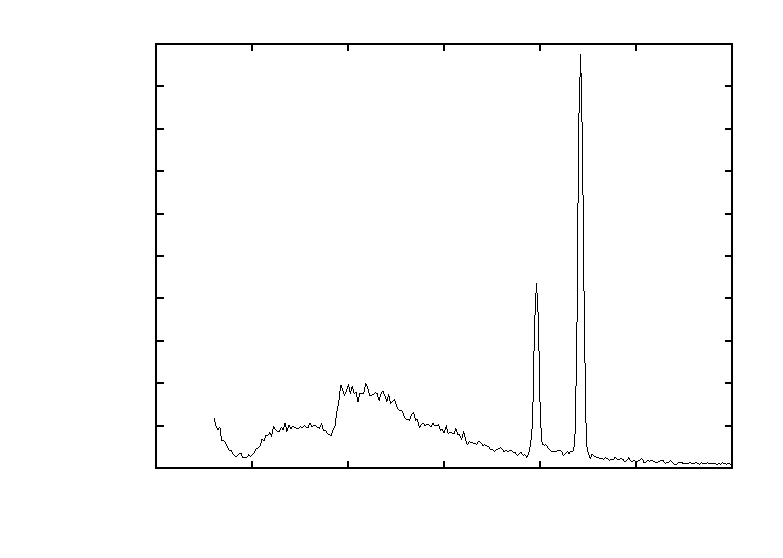
\includegraphics{Cu33Zr}}%
    \gplfronttext
  \end{picture}%
\endgroup

\end{center}
\caption{Spektrum rengenky s Cu anodou s Zr absorbérem při napětí 33 kV a expozicí 2 s.}
\end{figure}
\begin{figure}
\begin{center}
% GNUPLOT: LaTeX picture with Postscript
\begingroup
  \makeatletter
  \providecommand\color[2][]{%
    \GenericError{(gnuplot) \space\space\space\@spaces}{%
      Package color not loaded in conjunction with
      terminal option `colourtext'%
    }{See the gnuplot documentation for explanation.%
    }{Either use 'blacktext' in gnuplot or load the package
      color.sty in LaTeX.}%
    \renewcommand\color[2][]{}%
  }%
  \providecommand\includegraphics[2][]{%
    \GenericError{(gnuplot) \space\space\space\@spaces}{%
      Package graphicx or graphics not loaded%
    }{See the gnuplot documentation for explanation.%
    }{The gnuplot epslatex terminal needs graphicx.sty or graphics.sty.}%
    \renewcommand\includegraphics[2][]{}%
  }%
  \providecommand\rotatebox[2]{#2}%
  \@ifundefined{ifGPcolor}{%
    \newif\ifGPcolor
    \GPcolorfalse
  }{}%
  \@ifundefined{ifGPblacktext}{%
    \newif\ifGPblacktext
    \GPblacktexttrue
  }{}%
  % define a \g@addto@macro without @ in the name:
  \let\gplgaddtomacro\g@addto@macro
  % define empty templates for all commands taking text:
  \gdef\gplbacktext{}%
  \gdef\gplfronttext{}%
  \makeatother
  \ifGPblacktext
    % no textcolor at all
    \def\colorrgb#1{}%
    \def\colorgray#1{}%
  \else
    % gray or color?
    \ifGPcolor
      \def\colorrgb#1{\color[rgb]{#1}}%
      \def\colorgray#1{\color[gray]{#1}}%
      \expandafter\def\csname LTw\endcsname{\color{white}}%
      \expandafter\def\csname LTb\endcsname{\color{black}}%
      \expandafter\def\csname LTa\endcsname{\color{black}}%
      \expandafter\def\csname LT0\endcsname{\color[rgb]{1,0,0}}%
      \expandafter\def\csname LT1\endcsname{\color[rgb]{0,1,0}}%
      \expandafter\def\csname LT2\endcsname{\color[rgb]{0,0,1}}%
      \expandafter\def\csname LT3\endcsname{\color[rgb]{1,0,1}}%
      \expandafter\def\csname LT4\endcsname{\color[rgb]{0,1,1}}%
      \expandafter\def\csname LT5\endcsname{\color[rgb]{1,1,0}}%
      \expandafter\def\csname LT6\endcsname{\color[rgb]{0,0,0}}%
      \expandafter\def\csname LT7\endcsname{\color[rgb]{1,0.3,0}}%
      \expandafter\def\csname LT8\endcsname{\color[rgb]{0.5,0.5,0.5}}%
    \else
      % gray
      \def\colorrgb#1{\color{black}}%
      \def\colorgray#1{\color[gray]{#1}}%
      \expandafter\def\csname LTw\endcsname{\color{white}}%
      \expandafter\def\csname LTb\endcsname{\color{black}}%
      \expandafter\def\csname LTa\endcsname{\color{black}}%
      \expandafter\def\csname LT0\endcsname{\color{black}}%
      \expandafter\def\csname LT1\endcsname{\color{black}}%
      \expandafter\def\csname LT2\endcsname{\color{black}}%
      \expandafter\def\csname LT3\endcsname{\color{black}}%
      \expandafter\def\csname LT4\endcsname{\color{black}}%
      \expandafter\def\csname LT5\endcsname{\color{black}}%
      \expandafter\def\csname LT6\endcsname{\color{black}}%
      \expandafter\def\csname LT7\endcsname{\color{black}}%
      \expandafter\def\csname LT8\endcsname{\color{black}}%
    \fi
  \fi
  \setlength{\unitlength}{0.0500bp}%
  \begin{picture}(7200.00,5040.00)%
    \gplgaddtomacro\gplbacktext{%
      \csname LTb\endcsname%
      \put(1210,704){\makebox(0,0)[r]{\strut{} 0}}%
      \put(1210,1156){\makebox(0,0)[r]{\strut{} 500}}%
      \put(1210,1609){\makebox(0,0)[r]{\strut{} 1000}}%
      \put(1210,2061){\makebox(0,0)[r]{\strut{} 1500}}%
      \put(1210,2513){\makebox(0,0)[r]{\strut{} 2000}}%
      \put(1210,2966){\makebox(0,0)[r]{\strut{} 2500}}%
      \put(1210,3418){\makebox(0,0)[r]{\strut{} 3000}}%
      \put(1210,3870){\makebox(0,0)[r]{\strut{} 3500}}%
      \put(1210,4323){\makebox(0,0)[r]{\strut{} 4000}}%
      \put(1210,4775){\makebox(0,0)[r]{\strut{} 4500}}%
      \put(1342,484){\makebox(0,0){\strut{} 0}}%
      \put(2263,484){\makebox(0,0){\strut{} 5}}%
      \put(3184,484){\makebox(0,0){\strut{} 10}}%
      \put(4105,484){\makebox(0,0){\strut{} 15}}%
      \put(5027,484){\makebox(0,0){\strut{} 20}}%
      \put(5948,484){\makebox(0,0){\strut{} 25}}%
      \put(6869,484){\makebox(0,0){\strut{} 30}}%
      \put(308,2739){\rotatebox{-270}{\makebox(0,0){\strut{}Imp/s}}}%
      \put(4105,154){\makebox(0,0){\strut{}$\theta$/\st}}%
    }%
    \gplgaddtomacro\gplfronttext{%
    }%
    \gplbacktext
    \put(0,0){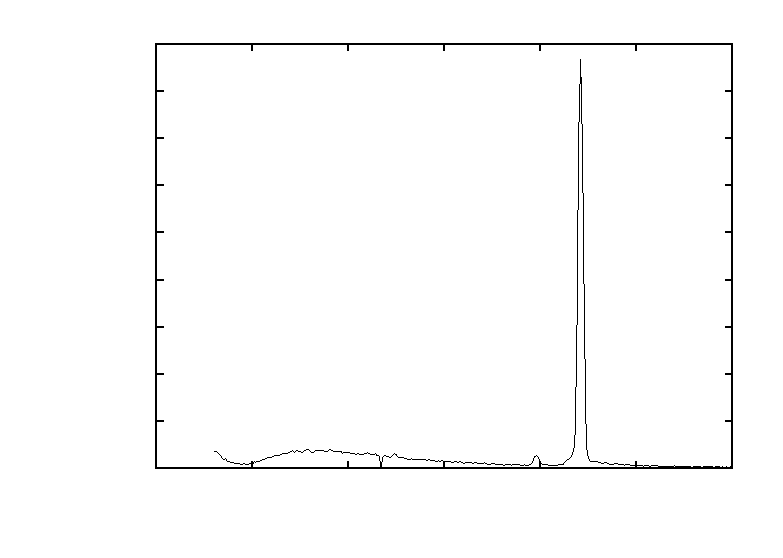
\includegraphics{Cu33Ni}}%
    \gplfronttext
  \end{picture}%
\endgroup

\end{center}
\caption{Spektrum rengenky s Cu anodou s Ni absorbérem při napětí 33 kV a expozicí 2 s.}
\end{figure}

\begin{figure}
\begin{center}
% GNUPLOT: LaTeX picture with Postscript
\begingroup
  \makeatletter
  \providecommand\color[2][]{%
    \GenericError{(gnuplot) \space\space\space\@spaces}{%
      Package color not loaded in conjunction with
      terminal option `colourtext'%
    }{See the gnuplot documentation for explanation.%
    }{Either use 'blacktext' in gnuplot or load the package
      color.sty in LaTeX.}%
    \renewcommand\color[2][]{}%
  }%
  \providecommand\includegraphics[2][]{%
    \GenericError{(gnuplot) \space\space\space\@spaces}{%
      Package graphicx or graphics not loaded%
    }{See the gnuplot documentation for explanation.%
    }{The gnuplot epslatex terminal needs graphicx.sty or graphics.sty.}%
    \renewcommand\includegraphics[2][]{}%
  }%
  \providecommand\rotatebox[2]{#2}%
  \@ifundefined{ifGPcolor}{%
    \newif\ifGPcolor
    \GPcolorfalse
  }{}%
  \@ifundefined{ifGPblacktext}{%
    \newif\ifGPblacktext
    \GPblacktexttrue
  }{}%
  % define a \g@addto@macro without @ in the name:
  \let\gplgaddtomacro\g@addto@macro
  % define empty templates for all commands taking text:
  \gdef\gplbacktext{}%
  \gdef\gplfronttext{}%
  \makeatother
  \ifGPblacktext
    % no textcolor at all
    \def\colorrgb#1{}%
    \def\colorgray#1{}%
  \else
    % gray or color?
    \ifGPcolor
      \def\colorrgb#1{\color[rgb]{#1}}%
      \def\colorgray#1{\color[gray]{#1}}%
      \expandafter\def\csname LTw\endcsname{\color{white}}%
      \expandafter\def\csname LTb\endcsname{\color{black}}%
      \expandafter\def\csname LTa\endcsname{\color{black}}%
      \expandafter\def\csname LT0\endcsname{\color[rgb]{1,0,0}}%
      \expandafter\def\csname LT1\endcsname{\color[rgb]{0,1,0}}%
      \expandafter\def\csname LT2\endcsname{\color[rgb]{0,0,1}}%
      \expandafter\def\csname LT3\endcsname{\color[rgb]{1,0,1}}%
      \expandafter\def\csname LT4\endcsname{\color[rgb]{0,1,1}}%
      \expandafter\def\csname LT5\endcsname{\color[rgb]{1,1,0}}%
      \expandafter\def\csname LT6\endcsname{\color[rgb]{0,0,0}}%
      \expandafter\def\csname LT7\endcsname{\color[rgb]{1,0.3,0}}%
      \expandafter\def\csname LT8\endcsname{\color[rgb]{0.5,0.5,0.5}}%
    \else
      % gray
      \def\colorrgb#1{\color{black}}%
      \def\colorgray#1{\color[gray]{#1}}%
      \expandafter\def\csname LTw\endcsname{\color{white}}%
      \expandafter\def\csname LTb\endcsname{\color{black}}%
      \expandafter\def\csname LTa\endcsname{\color{black}}%
      \expandafter\def\csname LT0\endcsname{\color{black}}%
      \expandafter\def\csname LT1\endcsname{\color{black}}%
      \expandafter\def\csname LT2\endcsname{\color{black}}%
      \expandafter\def\csname LT3\endcsname{\color{black}}%
      \expandafter\def\csname LT4\endcsname{\color{black}}%
      \expandafter\def\csname LT5\endcsname{\color{black}}%
      \expandafter\def\csname LT6\endcsname{\color{black}}%
      \expandafter\def\csname LT7\endcsname{\color{black}}%
      \expandafter\def\csname LT8\endcsname{\color{black}}%
    \fi
  \fi
  \setlength{\unitlength}{0.0500bp}%
  \begin{picture}(7200.00,5040.00)%
    \gplgaddtomacro\gplbacktext{%
      \csname LTb\endcsname%
      \put(1210,704){\makebox(0,0)[r]{\strut{} 0}}%
      \put(1210,1213){\makebox(0,0)[r]{\strut{} 500}}%
      \put(1210,1722){\makebox(0,0)[r]{\strut{} 1000}}%
      \put(1210,2231){\makebox(0,0)[r]{\strut{} 1500}}%
      \put(1210,2739){\makebox(0,0)[r]{\strut{} 2000}}%
      \put(1210,3248){\makebox(0,0)[r]{\strut{} 2500}}%
      \put(1210,3757){\makebox(0,0)[r]{\strut{} 3000}}%
      \put(1210,4266){\makebox(0,0)[r]{\strut{} 3500}}%
      \put(1210,4775){\makebox(0,0)[r]{\strut{} 4000}}%
      \put(1342,484){\makebox(0,0){\strut{} 0}}%
      \put(2263,484){\makebox(0,0){\strut{} 5}}%
      \put(3184,484){\makebox(0,0){\strut{} 10}}%
      \put(4105,484){\makebox(0,0){\strut{} 15}}%
      \put(5027,484){\makebox(0,0){\strut{} 20}}%
      \put(5948,484){\makebox(0,0){\strut{} 25}}%
      \put(6869,484){\makebox(0,0){\strut{} 30}}%
      \put(308,2739){\rotatebox{-270}{\makebox(0,0){\strut{}Imp/s}}}%
      \put(4105,154){\makebox(0,0){\strut{}$\theta$/\st}}%
    }%
    \gplgaddtomacro\gplfronttext{%
    }%
    \gplbacktext
    \put(0,0){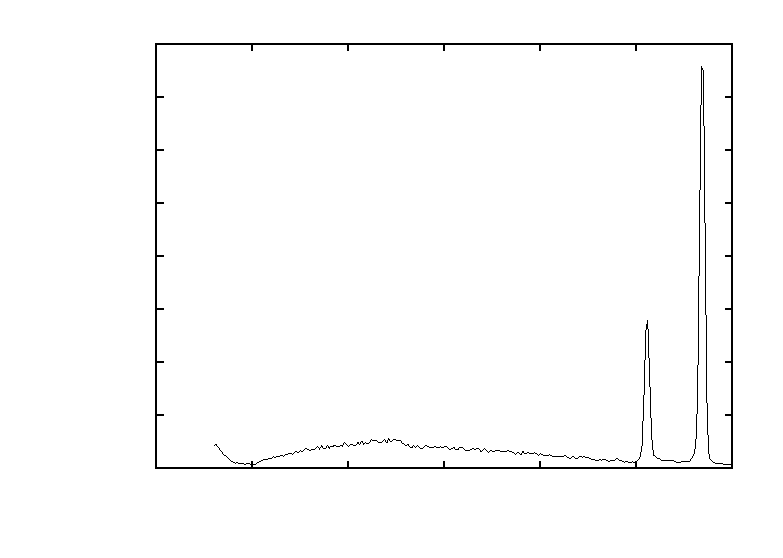
\includegraphics{Fe33}}%
    \gplfronttext
  \end{picture}%
\endgroup

\end{center}
\caption{Spektrum rengenky s Fe anodou při napětí 33 kV a expozicí 2 s.}
\end{figure}

\begin{figure}
\begin{center}
% GNUPLOT: LaTeX picture with Postscript
\begingroup
  \makeatletter
  \providecommand\color[2][]{%
    \GenericError{(gnuplot) \space\space\space\@spaces}{%
      Package color not loaded in conjunction with
      terminal option `colourtext'%
    }{See the gnuplot documentation for explanation.%
    }{Either use 'blacktext' in gnuplot or load the package
      color.sty in LaTeX.}%
    \renewcommand\color[2][]{}%
  }%
  \providecommand\includegraphics[2][]{%
    \GenericError{(gnuplot) \space\space\space\@spaces}{%
      Package graphicx or graphics not loaded%
    }{See the gnuplot documentation for explanation.%
    }{The gnuplot epslatex terminal needs graphicx.sty or graphics.sty.}%
    \renewcommand\includegraphics[2][]{}%
  }%
  \providecommand\rotatebox[2]{#2}%
  \@ifundefined{ifGPcolor}{%
    \newif\ifGPcolor
    \GPcolorfalse
  }{}%
  \@ifundefined{ifGPblacktext}{%
    \newif\ifGPblacktext
    \GPblacktexttrue
  }{}%
  % define a \g@addto@macro without @ in the name:
  \let\gplgaddtomacro\g@addto@macro
  % define empty templates for all commands taking text:
  \gdef\gplbacktext{}%
  \gdef\gplfronttext{}%
  \makeatother
  \ifGPblacktext
    % no textcolor at all
    \def\colorrgb#1{}%
    \def\colorgray#1{}%
  \else
    % gray or color?
    \ifGPcolor
      \def\colorrgb#1{\color[rgb]{#1}}%
      \def\colorgray#1{\color[gray]{#1}}%
      \expandafter\def\csname LTw\endcsname{\color{white}}%
      \expandafter\def\csname LTb\endcsname{\color{black}}%
      \expandafter\def\csname LTa\endcsname{\color{black}}%
      \expandafter\def\csname LT0\endcsname{\color[rgb]{1,0,0}}%
      \expandafter\def\csname LT1\endcsname{\color[rgb]{0,1,0}}%
      \expandafter\def\csname LT2\endcsname{\color[rgb]{0,0,1}}%
      \expandafter\def\csname LT3\endcsname{\color[rgb]{1,0,1}}%
      \expandafter\def\csname LT4\endcsname{\color[rgb]{0,1,1}}%
      \expandafter\def\csname LT5\endcsname{\color[rgb]{1,1,0}}%
      \expandafter\def\csname LT6\endcsname{\color[rgb]{0,0,0}}%
      \expandafter\def\csname LT7\endcsname{\color[rgb]{1,0.3,0}}%
      \expandafter\def\csname LT8\endcsname{\color[rgb]{0.5,0.5,0.5}}%
    \else
      % gray
      \def\colorrgb#1{\color{black}}%
      \def\colorgray#1{\color[gray]{#1}}%
      \expandafter\def\csname LTw\endcsname{\color{white}}%
      \expandafter\def\csname LTb\endcsname{\color{black}}%
      \expandafter\def\csname LTa\endcsname{\color{black}}%
      \expandafter\def\csname LT0\endcsname{\color{black}}%
      \expandafter\def\csname LT1\endcsname{\color{black}}%
      \expandafter\def\csname LT2\endcsname{\color{black}}%
      \expandafter\def\csname LT3\endcsname{\color{black}}%
      \expandafter\def\csname LT4\endcsname{\color{black}}%
      \expandafter\def\csname LT5\endcsname{\color{black}}%
      \expandafter\def\csname LT6\endcsname{\color{black}}%
      \expandafter\def\csname LT7\endcsname{\color{black}}%
      \expandafter\def\csname LT8\endcsname{\color{black}}%
    \fi
  \fi
  \setlength{\unitlength}{0.0500bp}%
  \begin{picture}(7200.00,5040.00)%
    \gplgaddtomacro\gplbacktext{%
      \csname LTb\endcsname%
      \put(1078,704){\makebox(0,0)[r]{\strut{} 0}}%
      \put(1078,1111){\makebox(0,0)[r]{\strut{} 20}}%
      \put(1078,1518){\makebox(0,0)[r]{\strut{} 40}}%
      \put(1078,1925){\makebox(0,0)[r]{\strut{} 60}}%
      \put(1078,2332){\makebox(0,0)[r]{\strut{} 80}}%
      \put(1078,2740){\makebox(0,0)[r]{\strut{} 100}}%
      \put(1078,3147){\makebox(0,0)[r]{\strut{} 120}}%
      \put(1078,3554){\makebox(0,0)[r]{\strut{} 140}}%
      \put(1078,3961){\makebox(0,0)[r]{\strut{} 160}}%
      \put(1078,4368){\makebox(0,0)[r]{\strut{} 180}}%
      \put(1078,4775){\makebox(0,0)[r]{\strut{} 200}}%
      \put(1210,484){\makebox(0,0){\strut{} 0}}%
      \put(2153,484){\makebox(0,0){\strut{} 5}}%
      \put(3096,484){\makebox(0,0){\strut{} 10}}%
      \put(4039,484){\makebox(0,0){\strut{} 15}}%
      \put(4983,484){\makebox(0,0){\strut{} 20}}%
      \put(5926,484){\makebox(0,0){\strut{} 25}}%
      \put(6869,484){\makebox(0,0){\strut{} 30}}%
      \put(308,2739){\rotatebox{-270}{\makebox(0,0){\strut{}Imp/s}}}%
      \put(4039,154){\makebox(0,0){\strut{}$\theta$/\st}}%
    }%
    \gplgaddtomacro\gplfronttext{%
    }%
    \gplbacktext
    \put(0,0){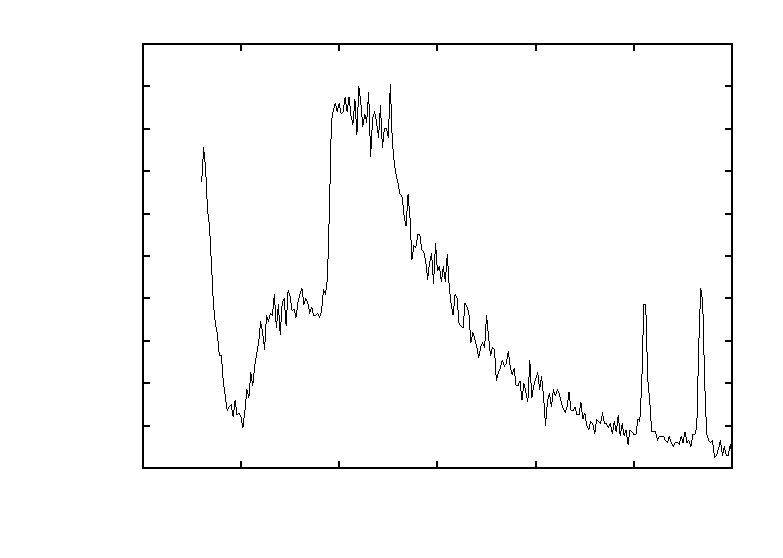
\includegraphics{Fe33Zr}}%
    \gplfronttext
  \end{picture}%
\endgroup

\end{center}
\caption{Spektrum rengenky s Fe anodou s Zr absorbérem při napětí 33 kV a expozicí 2 s.}
\end{figure}

\begin{figure}
\begin{center}
% GNUPLOT: LaTeX picture with Postscript
\begingroup
  \makeatletter
  \providecommand\color[2][]{%
    \GenericError{(gnuplot) \space\space\space\@spaces}{%
      Package color not loaded in conjunction with
      terminal option `colourtext'%
    }{See the gnuplot documentation for explanation.%
    }{Either use 'blacktext' in gnuplot or load the package
      color.sty in LaTeX.}%
    \renewcommand\color[2][]{}%
  }%
  \providecommand\includegraphics[2][]{%
    \GenericError{(gnuplot) \space\space\space\@spaces}{%
      Package graphicx or graphics not loaded%
    }{See the gnuplot documentation for explanation.%
    }{The gnuplot epslatex terminal needs graphicx.sty or graphics.sty.}%
    \renewcommand\includegraphics[2][]{}%
  }%
  \providecommand\rotatebox[2]{#2}%
  \@ifundefined{ifGPcolor}{%
    \newif\ifGPcolor
    \GPcolorfalse
  }{}%
  \@ifundefined{ifGPblacktext}{%
    \newif\ifGPblacktext
    \GPblacktexttrue
  }{}%
  % define a \g@addto@macro without @ in the name:
  \let\gplgaddtomacro\g@addto@macro
  % define empty templates for all commands taking text:
  \gdef\gplbacktext{}%
  \gdef\gplfronttext{}%
  \makeatother
  \ifGPblacktext
    % no textcolor at all
    \def\colorrgb#1{}%
    \def\colorgray#1{}%
  \else
    % gray or color?
    \ifGPcolor
      \def\colorrgb#1{\color[rgb]{#1}}%
      \def\colorgray#1{\color[gray]{#1}}%
      \expandafter\def\csname LTw\endcsname{\color{white}}%
      \expandafter\def\csname LTb\endcsname{\color{black}}%
      \expandafter\def\csname LTa\endcsname{\color{black}}%
      \expandafter\def\csname LT0\endcsname{\color[rgb]{1,0,0}}%
      \expandafter\def\csname LT1\endcsname{\color[rgb]{0,1,0}}%
      \expandafter\def\csname LT2\endcsname{\color[rgb]{0,0,1}}%
      \expandafter\def\csname LT3\endcsname{\color[rgb]{1,0,1}}%
      \expandafter\def\csname LT4\endcsname{\color[rgb]{0,1,1}}%
      \expandafter\def\csname LT5\endcsname{\color[rgb]{1,1,0}}%
      \expandafter\def\csname LT6\endcsname{\color[rgb]{0,0,0}}%
      \expandafter\def\csname LT7\endcsname{\color[rgb]{1,0.3,0}}%
      \expandafter\def\csname LT8\endcsname{\color[rgb]{0.5,0.5,0.5}}%
    \else
      % gray
      \def\colorrgb#1{\color{black}}%
      \def\colorgray#1{\color[gray]{#1}}%
      \expandafter\def\csname LTw\endcsname{\color{white}}%
      \expandafter\def\csname LTb\endcsname{\color{black}}%
      \expandafter\def\csname LTa\endcsname{\color{black}}%
      \expandafter\def\csname LT0\endcsname{\color{black}}%
      \expandafter\def\csname LT1\endcsname{\color{black}}%
      \expandafter\def\csname LT2\endcsname{\color{black}}%
      \expandafter\def\csname LT3\endcsname{\color{black}}%
      \expandafter\def\csname LT4\endcsname{\color{black}}%
      \expandafter\def\csname LT5\endcsname{\color{black}}%
      \expandafter\def\csname LT6\endcsname{\color{black}}%
      \expandafter\def\csname LT7\endcsname{\color{black}}%
      \expandafter\def\csname LT8\endcsname{\color{black}}%
    \fi
  \fi
  \setlength{\unitlength}{0.0500bp}%
  \begin{picture}(7200.00,5040.00)%
    \gplgaddtomacro\gplbacktext{%
      \csname LTb\endcsname%
      \put(1210,704){\makebox(0,0)[r]{\strut{} 0}}%
      \put(1210,1382){\makebox(0,0)[r]{\strut{} 500}}%
      \put(1210,2061){\makebox(0,0)[r]{\strut{} 1000}}%
      \put(1210,2739){\makebox(0,0)[r]{\strut{} 1500}}%
      \put(1210,3418){\makebox(0,0)[r]{\strut{} 2000}}%
      \put(1210,4096){\makebox(0,0)[r]{\strut{} 2500}}%
      \put(1210,4775){\makebox(0,0)[r]{\strut{} 3000}}%
      \put(1342,484){\makebox(0,0){\strut{} 0}}%
      \put(2132,484){\makebox(0,0){\strut{} 5}}%
      \put(2921,484){\makebox(0,0){\strut{} 10}}%
      \put(3711,484){\makebox(0,0){\strut{} 15}}%
      \put(4500,484){\makebox(0,0){\strut{} 20}}%
      \put(5290,484){\makebox(0,0){\strut{} 25}}%
      \put(6079,484){\makebox(0,0){\strut{} 30}}%
      \put(6869,484){\makebox(0,0){\strut{} 35}}%
      \put(308,2739){\rotatebox{-270}{\makebox(0,0){\strut{}Imp/s}}}%
      \put(4105,154){\makebox(0,0){\strut{}$\theta$/\st}}%
    }%
    \gplgaddtomacro\gplfronttext{%
    }%
    \gplbacktext
    \put(0,0){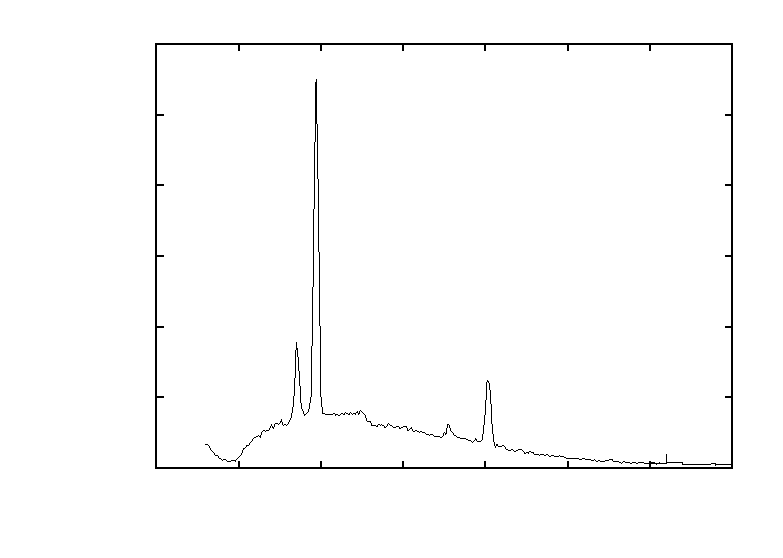
\includegraphics{Mo33}}%
    \gplfronttext
  \end{picture}%
\endgroup

\end{center}
\caption{Spektrum rengenky s Mo anodou při napětí 33 kV a expozicí 3 s.}
\end{figure}

\begin{figure}
\begin{center}
% GNUPLOT: LaTeX picture with Postscript
\begingroup
  \makeatletter
  \providecommand\color[2][]{%
    \GenericError{(gnuplot) \space\space\space\@spaces}{%
      Package color not loaded in conjunction with
      terminal option `colourtext'%
    }{See the gnuplot documentation for explanation.%
    }{Either use 'blacktext' in gnuplot or load the package
      color.sty in LaTeX.}%
    \renewcommand\color[2][]{}%
  }%
  \providecommand\includegraphics[2][]{%
    \GenericError{(gnuplot) \space\space\space\@spaces}{%
      Package graphicx or graphics not loaded%
    }{See the gnuplot documentation for explanation.%
    }{The gnuplot epslatex terminal needs graphicx.sty or graphics.sty.}%
    \renewcommand\includegraphics[2][]{}%
  }%
  \providecommand\rotatebox[2]{#2}%
  \@ifundefined{ifGPcolor}{%
    \newif\ifGPcolor
    \GPcolorfalse
  }{}%
  \@ifundefined{ifGPblacktext}{%
    \newif\ifGPblacktext
    \GPblacktexttrue
  }{}%
  % define a \g@addto@macro without @ in the name:
  \let\gplgaddtomacro\g@addto@macro
  % define empty templates for all commands taking text:
  \gdef\gplbacktext{}%
  \gdef\gplfronttext{}%
  \makeatother
  \ifGPblacktext
    % no textcolor at all
    \def\colorrgb#1{}%
    \def\colorgray#1{}%
  \else
    % gray or color?
    \ifGPcolor
      \def\colorrgb#1{\color[rgb]{#1}}%
      \def\colorgray#1{\color[gray]{#1}}%
      \expandafter\def\csname LTw\endcsname{\color{white}}%
      \expandafter\def\csname LTb\endcsname{\color{black}}%
      \expandafter\def\csname LTa\endcsname{\color{black}}%
      \expandafter\def\csname LT0\endcsname{\color[rgb]{1,0,0}}%
      \expandafter\def\csname LT1\endcsname{\color[rgb]{0,1,0}}%
      \expandafter\def\csname LT2\endcsname{\color[rgb]{0,0,1}}%
      \expandafter\def\csname LT3\endcsname{\color[rgb]{1,0,1}}%
      \expandafter\def\csname LT4\endcsname{\color[rgb]{0,1,1}}%
      \expandafter\def\csname LT5\endcsname{\color[rgb]{1,1,0}}%
      \expandafter\def\csname LT6\endcsname{\color[rgb]{0,0,0}}%
      \expandafter\def\csname LT7\endcsname{\color[rgb]{1,0.3,0}}%
      \expandafter\def\csname LT8\endcsname{\color[rgb]{0.5,0.5,0.5}}%
    \else
      % gray
      \def\colorrgb#1{\color{black}}%
      \def\colorgray#1{\color[gray]{#1}}%
      \expandafter\def\csname LTw\endcsname{\color{white}}%
      \expandafter\def\csname LTb\endcsname{\color{black}}%
      \expandafter\def\csname LTa\endcsname{\color{black}}%
      \expandafter\def\csname LT0\endcsname{\color{black}}%
      \expandafter\def\csname LT1\endcsname{\color{black}}%
      \expandafter\def\csname LT2\endcsname{\color{black}}%
      \expandafter\def\csname LT3\endcsname{\color{black}}%
      \expandafter\def\csname LT4\endcsname{\color{black}}%
      \expandafter\def\csname LT5\endcsname{\color{black}}%
      \expandafter\def\csname LT6\endcsname{\color{black}}%
      \expandafter\def\csname LT7\endcsname{\color{black}}%
      \expandafter\def\csname LT8\endcsname{\color{black}}%
    \fi
  \fi
  \setlength{\unitlength}{0.0500bp}%
  \begin{picture}(7200.00,5040.00)%
    \gplgaddtomacro\gplbacktext{%
      \csname LTb\endcsname%
      \put(1210,704){\makebox(0,0)[r]{\strut{} 0}}%
      \put(1210,1383){\makebox(0,0)[r]{\strut{} 200}}%
      \put(1210,2061){\makebox(0,0)[r]{\strut{} 400}}%
      \put(1210,2740){\makebox(0,0)[r]{\strut{} 600}}%
      \put(1210,3418){\makebox(0,0)[r]{\strut{} 800}}%
      \put(1210,4097){\makebox(0,0)[r]{\strut{} 1000}}%
      \put(1210,4775){\makebox(0,0)[r]{\strut{} 1200}}%
      \put(1342,484){\makebox(0,0){\strut{} 42}}%
      \put(1956,484){\makebox(0,0){\strut{} 43}}%
      \put(2570,484){\makebox(0,0){\strut{} 44}}%
      \put(3184,484){\makebox(0,0){\strut{} 45}}%
      \put(3798,484){\makebox(0,0){\strut{} 46}}%
      \put(4413,484){\makebox(0,0){\strut{} 47}}%
      \put(5027,484){\makebox(0,0){\strut{} 48}}%
      \put(5641,484){\makebox(0,0){\strut{} 49}}%
      \put(6255,484){\makebox(0,0){\strut{} 50}}%
      \put(6869,484){\makebox(0,0){\strut{} 51}}%
      \put(308,2739){\rotatebox{-270}{\makebox(0,0){\strut{}Imp/s}}}%
      \put(4105,154){\makebox(0,0){\strut{}$\theta$/\st}}%
    }%
    \gplgaddtomacro\gplfronttext{%
    }%
    \gplbacktext
    \put(0,0){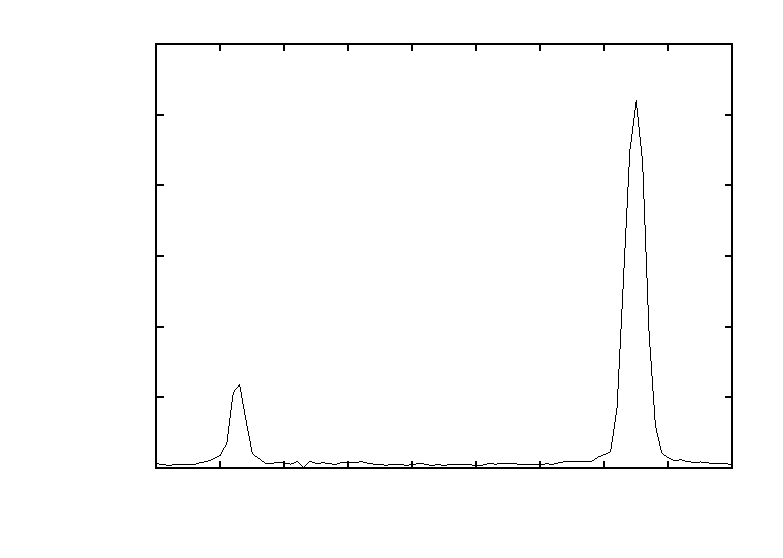
\includegraphics{Cu33n2}}%
    \gplfronttext
  \end{picture}%
\endgroup

\end{center}
\caption{Spektrum rengenky s Cu anodou při napětí 33 kV a expozicí 2 s.}
\label{posledni}
\end{figure}

\subsection{Planckova konstanta}
Pro každý  druh rengenky jsem odečetů z grafu mezní hranici brzdné části spektra $\theta_m$. 
\begin{eqnarray}
\theta_{mCu}=(4.6 \pm 0.3)^{\circ} \\
\theta_{mFe}=(4.7 \pm 0.3)^{\circ} \\
\theta_{mMo}=(4.6 \pm 0.3)^{\circ}
\end{eqnarray}
Z té jsem dle Braggova zákona \ref{bragg} dopočítal $\lambda$
\begin{eqnarray}
\lambda=(32 \pm 3) \mbox{pm},
\end{eqnarray}
kterou jsem dosadil do rovnice \ref{planc} a získal
\begin{eqnarray}
h=(5.7 \pm 1.2)\cdot 10^{-34} \mbox{Js}
\end{eqnarray}
Pro srovnaní tabelová hodnota je
\begin{eqnarray}
h=6.6\cdot10^{-34} \mbox{Js}
\end{eqnarray}

\subsection{Moseleyův zákon}
Nejprve jsem z namměřených spekter odečetl specifické délky záření
\begin{eqnarray}
K_{Cu\beta}=(135.8 \pm 0.2)^{\circ} \mbox{pm}\\
K_{Cu\alpha}=(151.5 \pm 0.2)^{\circ} \mbox{pm}\\
K_{Fe\beta}=(173.4 \pm 0.2)^{\circ} \mbox{pm}\\
K_{Fe\alpha}=(191.6 \pm 0.2)^{\circ} \mbox{pm}\\
K_{Mo\beta}=(59.5 \pm 0.2)^{\circ} \mbox{pm}\\
K_{Mo\alpha}=(67.9 \pm 0.2)^{\circ} \mbox{pm}\\
K_{Mo2\beta}=(122.5 \pm 0.2)^{\circ} \mbox{pm}\\
K_{Mo2\alpha}=(139.0 \pm 0.2)^{\circ} \mbox{pm}
\end{eqnarray}
Hodnoty pro alpha jsem přepočítal a vyneslu na obrázlu \ref{kal} jako závislost $\sqrt{\omega}$ na Z. Tyto hodnoty jsem proložil přímkou a ze směrnice dopočetl
\begin{eqnarray}
R_\omega=(2.37\pm0.05) \mbox{s}^{-1}
\end{eqnarray}
Stínění vyšlo
\begin{eqnarray}
s=2.5\pm0.3
\end{eqnarray}
Po dosazení těchto hodnot do Moseleyova zákonu se ná snadno ověřit i jeho platnost pro absobční hrany.

Porovnáním intenzit pro $K_Cu\beta$ získáme filtrační efekt Niklu pro tuto $\lambda$
\begin{eqnarray}
F=(93 \pm 1)\%.
\end{eqnarray}

\begin{figure}
\begin{center}
% GNUPLOT: LaTeX picture with Postscript
\begingroup
  \makeatletter
  \providecommand\color[2][]{%
    \GenericError{(gnuplot) \space\space\space\@spaces}{%
      Package color not loaded in conjunction with
      terminal option `colourtext'%
    }{See the gnuplot documentation for explanation.%
    }{Either use 'blacktext' in gnuplot or load the package
      color.sty in LaTeX.}%
    \renewcommand\color[2][]{}%
  }%
  \providecommand\includegraphics[2][]{%
    \GenericError{(gnuplot) \space\space\space\@spaces}{%
      Package graphicx or graphics not loaded%
    }{See the gnuplot documentation for explanation.%
    }{The gnuplot epslatex terminal needs graphicx.sty or graphics.sty.}%
    \renewcommand\includegraphics[2][]{}%
  }%
  \providecommand\rotatebox[2]{#2}%
  \@ifundefined{ifGPcolor}{%
    \newif\ifGPcolor
    \GPcolorfalse
  }{}%
  \@ifundefined{ifGPblacktext}{%
    \newif\ifGPblacktext
    \GPblacktexttrue
  }{}%
  % define a \g@addto@macro without @ in the name:
  \let\gplgaddtomacro\g@addto@macro
  % define empty templates for all commands taking text:
  \gdef\gplbacktext{}%
  \gdef\gplfronttext{}%
  \makeatother
  \ifGPblacktext
    % no textcolor at all
    \def\colorrgb#1{}%
    \def\colorgray#1{}%
  \else
    % gray or color?
    \ifGPcolor
      \def\colorrgb#1{\color[rgb]{#1}}%
      \def\colorgray#1{\color[gray]{#1}}%
      \expandafter\def\csname LTw\endcsname{\color{white}}%
      \expandafter\def\csname LTb\endcsname{\color{black}}%
      \expandafter\def\csname LTa\endcsname{\color{black}}%
      \expandafter\def\csname LT0\endcsname{\color[rgb]{1,0,0}}%
      \expandafter\def\csname LT1\endcsname{\color[rgb]{0,1,0}}%
      \expandafter\def\csname LT2\endcsname{\color[rgb]{0,0,1}}%
      \expandafter\def\csname LT3\endcsname{\color[rgb]{1,0,1}}%
      \expandafter\def\csname LT4\endcsname{\color[rgb]{0,1,1}}%
      \expandafter\def\csname LT5\endcsname{\color[rgb]{1,1,0}}%
      \expandafter\def\csname LT6\endcsname{\color[rgb]{0,0,0}}%
      \expandafter\def\csname LT7\endcsname{\color[rgb]{1,0.3,0}}%
      \expandafter\def\csname LT8\endcsname{\color[rgb]{0.5,0.5,0.5}}%
    \else
      % gray
      \def\colorrgb#1{\color{black}}%
      \def\colorgray#1{\color[gray]{#1}}%
      \expandafter\def\csname LTw\endcsname{\color{white}}%
      \expandafter\def\csname LTb\endcsname{\color{black}}%
      \expandafter\def\csname LTa\endcsname{\color{black}}%
      \expandafter\def\csname LT0\endcsname{\color{black}}%
      \expandafter\def\csname LT1\endcsname{\color{black}}%
      \expandafter\def\csname LT2\endcsname{\color{black}}%
      \expandafter\def\csname LT3\endcsname{\color{black}}%
      \expandafter\def\csname LT4\endcsname{\color{black}}%
      \expandafter\def\csname LT5\endcsname{\color{black}}%
      \expandafter\def\csname LT6\endcsname{\color{black}}%
      \expandafter\def\csname LT7\endcsname{\color{black}}%
      \expandafter\def\csname LT8\endcsname{\color{black}}%
    \fi
  \fi
  \setlength{\unitlength}{0.0500bp}%
  \begin{picture}(7200.00,5040.00)%
    \gplgaddtomacro\gplbacktext{%
      \csname LTb\endcsname%
      \put(594,440){\makebox(0,0)[r]{\strut{} 0}}%
      \put(594,874){\makebox(0,0)[r]{\strut{} 1}}%
      \put(594,1307){\makebox(0,0)[r]{\strut{} 2}}%
      \put(594,1741){\makebox(0,0)[r]{\strut{} 3}}%
      \put(594,2174){\makebox(0,0)[r]{\strut{} 4}}%
      \put(594,2608){\makebox(0,0)[r]{\strut{} 5}}%
      \put(594,3041){\makebox(0,0)[r]{\strut{} 6}}%
      \put(594,3475){\makebox(0,0)[r]{\strut{} 7}}%
      \put(594,3908){\makebox(0,0)[r]{\strut{} 8}}%
      \put(594,4342){\makebox(0,0)[r]{\strut{} 9}}%
      \put(594,4775){\makebox(0,0)[r]{\strut{} 10}}%
      \put(726,220){\makebox(0,0){\strut{} 0}}%
      \put(1486,220){\makebox(0,0){\strut{} 0.2}}%
      \put(2245,220){\makebox(0,0){\strut{} 0.4}}%
      \put(3005,220){\makebox(0,0){\strut{} 0.6}}%
      \put(3765,220){\makebox(0,0){\strut{} 0.8}}%
      \put(4524,220){\makebox(0,0){\strut{} 1}}%
      \put(5284,220){\makebox(0,0){\strut{} 1.2}}%
      \put(6043,220){\makebox(0,0){\strut{} 1.4}}%
      \put(6803,220){\makebox(0,0){\strut{} 1.6}}%
    }%
    \gplgaddtomacro\gplfronttext{%
      \csname LTb\endcsname%
      \put(5816,613){\makebox(0,0)[r]{\strut{}kalibrační křivka}}%
    }%
    \gplbacktext
    \put(0,0){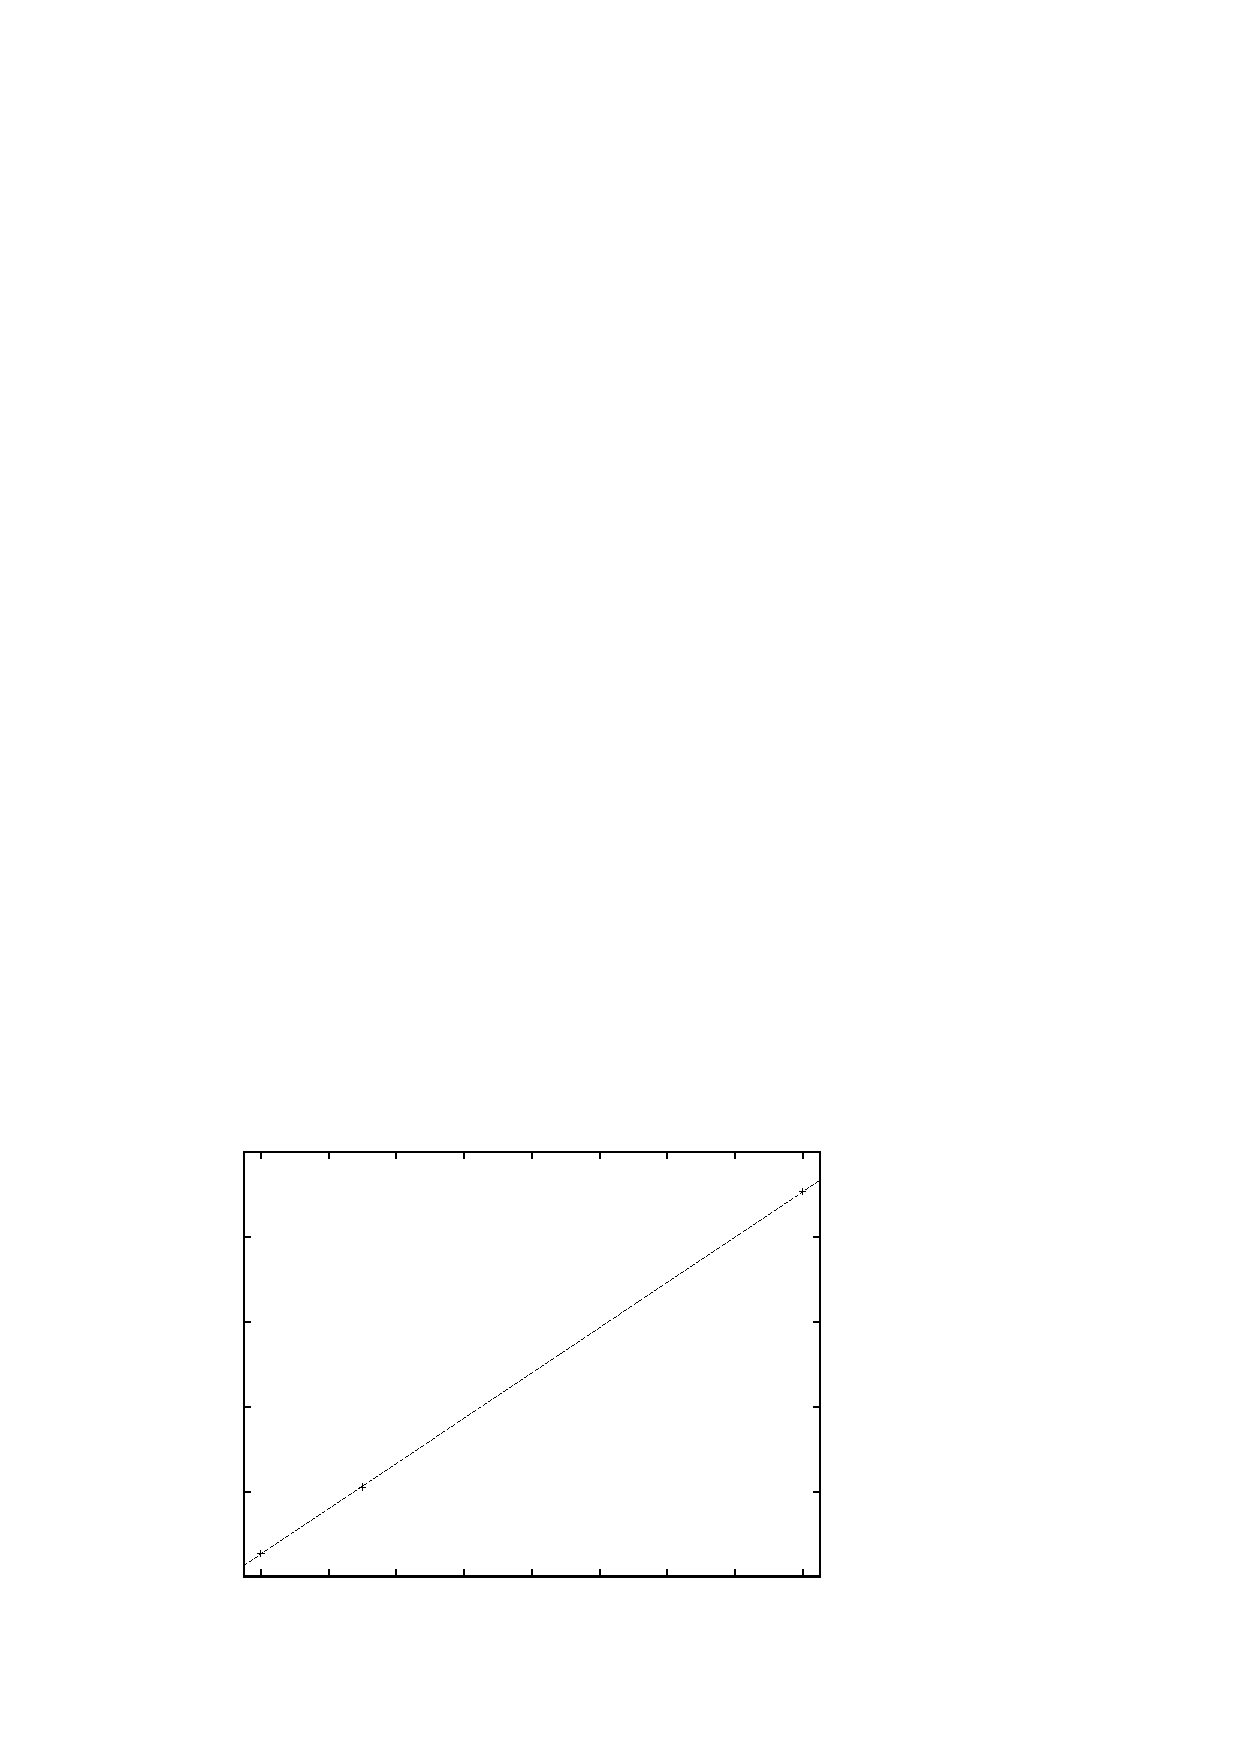
\includegraphics{kal}}%
    \gplfronttext
  \end{picture}%
\endgroup

\end{center}
\caption{Graf závislost $\sqrt{\omega}$ na Z pro $K_\alpha$}
\label{kal}
\end{figure}

\subsection{Úhlová disperze}
Z naměřeného spektra rengenky s Mo anodou jsem určil úhlovou disperzi pro prví a druhý řád dosazením do vztahu \ref{disp}.
\begin{eqnarray}
d_{n1}=(2.52 \pm 0.03)\cdot 10^9 \mbox{m}^{-1}\\
d_{n2}=(2.64 \pm 0.06)\cdot 10^9 \mbox{m}^{-1}
\end{eqnarray}

\section{Diskuze}
Naměřená spektra dopadla dle teoretických předpokladů. Jedinou odchylkou byly úhly odolo nuly. Vzhledem k uspořádání ecperimentu totiž docházelo k průchodu záření na detektor bez 
interakce s krystalem. Tento efekt zvýšil nepřesnost určení $\lambda_m$, protože se lehce překrýval s okolím této hodnoty. To má za následek velkou chybu určení Planckovy konstanty.
Ostatní počítané charakteristiky mají chybu o řád nižší, protože naměřené píky byli velmi úzké.

Poněkud ojedinělou chybou byl náhlý pokles intenzity pro určitou hodnotu na nulu. Tato chyba se neprojevovala nijak pravidelně a zřejmě se jedná pouze o ztrátu dat z detektoru. 

\section{Závěř}
\noindent
Proměřil jsem všechna spektra ze zadání. Výsledky jsou na obrázcích (\ref{prvni}) až (\ref{posledni}).\\
Určil jsem hodnotu Planckovy konstanty
\begin{eqnarray}
h=(5.7 \pm 1.2)\cdot 10^{-34} \mbox{Js}
\end{eqnarray}
Ověřil jsem platnost Moseleyova zákonu a určil hodnotu
\begin{eqnarray}
R_\omega=(2.37\pm0.05) \mbox{s}^{-1}
\end{eqnarray}
Ze spektra Mo anody jsem určil úhlovou disperzi
\begin{eqnarray}
d_{n1}=(2.52 \pm 0.03)\cdot10^{9} \mbox{m}^{-1}\\
d_{n2}=(2.64 \pm 0.06)\cdot10^{9} \mbox{m}^{-1}
\end{eqnarray}

\begin{thebibliography}{5}
	\bibitem{text} \textbf{Studijní text na praktikum IV} \\http://physics.mff.cuni.cz/vyuka/zfp/txt\_421.pdf (10. 11. 2012)
    \bibitem{chyba} \emph{J. Englich}: \textbf{Zpracování výsldků fyzikálních měření} \\ LS 1999/2000
\end{thebibliography}
\end{document}
